\documentclass[twoside]{book}
%\usepackage{algorithmic}
%\usepackage{eepic}
%\usepackage{epic}
\usepackage{amsmath}
\usepackage{amssymb}

\usepackage{latexsym}
\usepackage{times}
\usepackage{mathptm}
\usepackage{bbold}
\usepackage{comment}
\usepackage{epsfig}
%\usepackage{fancyheadings}
\usepackage{fancyhdr}
\usepackage{float}
\usepackage{floatflt}
\usepackage{graphics}
\usepackage{moreverb}
\usepackage{epic}
\usepackage{eepic}
\usepackage{theorem}
\usepackage{url}
%\usepackage{html}
\usepackage{listings}

\hoffset=-1in
\voffset=-1in
%-- Textbreite
\setlength{\textwidth}{120mm}           % 9/12 * 160mm
\setlength{\oddsidemargin}{23.3mm}      % 1/12 * 160mm + 10 ungesehene
\setlength{\evensidemargin}{26.6mm}     % 2/12 * 160mm
%-- Texthoehe
%\setlength{\textheight}{180mm}          % 9/12 * 240mm
\setlength{\textheight}{220mm}          % 9/12 * 240mm
\setlength{\topmargin}{20mm}            % 1/12 * 240mm


\addtolength{\textheight}{-\headheight}
\addtolength{\textheight}{-\headsep}

\hfuzz 1.5pt
\renewcommand{\topfraction}{0.999}
\renewcommand{\bottomfraction}{0.999}
\renewcommand{\textfraction}{0.001}


\pagestyle{fancyplain}

\renewcommand{\chaptermark}[1]{\markboth{#1}{#1}}
\renewcommand{\sectionmark}[1]{\markright{\thesection\ #1}}
\lhead[\fancyplain{{\tiny Dementiev \today} \bf\thepage}{\bf\thepage}]{
\fancyplain{\rightmark}}
\rhead[\fancyplain{}{\leftmark}]{\fancyplain{{\tiny Dementiev \today}
\bf\thepage}{\bf\thepage}} 
\cfoot[{\fancyplain{}{}}]{\fancyplain{}{}}

\renewcommand{\labelenumi}{\alph{enumi})}

% Peter's Makros
\newcommand{\Id}[1]{\ensuremath{\mathit{#1}}}
\newcommand{\vek}[1]{\mathbf{#1}}
\newcommand{\mat}[1]{\mathbf{#1}}
\newcommand{\ceil}[1]{\left\lceil #1\right\rceil}
\newcommand{\floor}[1]{\left\lfloor #1\right\rfloor}
\newcommand{\abs}[1]{\left| #1\right|}
\newcommand{\norm}[1]{\left\|#1\right\|}
\newcommand{\enorm}[1]{\norm{#1}_{2}}
\newcommand{\sumnorm}[1]{\norm{#1}_{1}}
\newcommand{\maxnorm}[1]{\norm{#1}_{\infty}}
\newcommand{\xor}{\oplus}
\newcommand{\set}[1]{\left\{ #1\right\}}
\newcommand{\sset}[1]{\set{#1}} % synomym?
\newcommand{\gilt}{:}
%\newcommand{\sodass}{\,:\,}
\newcommand{\sodass}{\mid}
\newcommand{\setGilt}[2]{\left\{ #1\gilt #2\right\}}
\newcommand{\seqGilt}[2]{\left\langle #1\gilt #2\right\rangle}
\newcommand{\Litem}[1]{\seq{#1}}
\newcommand{\Def}{:=}
\newcommand{\zvektor}[2]{\left(#1,#2\right)}
\newcommand{\vektor}[2]{\left(\begin{smallmatrix}#1\\#2\end{smallmatrix}\right)}
\newcommand{\vektord}[3]{\left(\begin{smallmatrix}#1\\#2\\#3\end{smallmatrix}\right)}
\newcommand{\condition}[1]{\left[#1\right]}
\newcommand{\binomial}[2]{\binom{#1}{#2}}
\newcommand{\even}{\mathrm{even}}
\newcommand{\odd}{\mathrm{odd}}
\newcommand{\mymod}{\,\bmod\,}
% \newcommand{\divides}{|}
%\newcommand{\Div}{\,\mathrm{div}\,}

% Typen
\newcommand{\nat}{\mathbb{N}}
\newcommand{\natnull}{\mathbb{N}_{0}}
\newcommand{\natplus}{\mathbb{N}_{+}}
%\newcommand{\natless}[1]{\mathbb{N}_{<#1}}
\newcommand{\natless}[1]{\mathbb{N}_{#1}}
\newcommand{\nplus}{\mathbb{N}_+}
\newcommand{\real}{\mathbb{R}}
\newcommand{\rplus}{\mathbb{R}_+}
\newcommand{\rnneg}{\mathbb{R}_*}
\newcommand{\integer}{\mathbb{Z}}
% \newcommand{\intint}[2]{\set{#1,\ldots, #2}}
\newcommand{\intint}[2]{{#1}..{#2}}
\newcommand{\realrange}[2]{\left[#1, #2\right]}
\newcommand{\realrangeo}[2]{\left(#1, #2\right)}
\newcommand{\realrangelo}[2]{\left(#1, #2\right]}
\newcommand{\realrangero}[2]{\left[#1, #2\right)}
\newcommand{\unitrange}[2]{\realrange{0}{1}}
\newcommand{\bool}{\set{0,1}}
%\newcommand{\boolean}{\mathbb{B}}
%\newcommand{\mapping}[2]{#1\rightarrow #2}
\newcommand{\mapping}[2]{{#2}^{#1}}
\newcommand{\powerset}[1]{{\cal P}\left(#1\right)}
\newcommand{\NP}{\mathbf{NP}}
\newcommand{\Bild}{\mathbf{Bild}\:}

% Typannotation
\newcommand{\withtype}[1]{\in#1}

% Wahrscheinlichkeitsrechnung
\newcommand{\condprob}[2]{{\mathbb{P}}\left(#1\;|\;#2\right)}
\newcommand{\condexpect}[2]{{\mathbb{E}}\left(#1\;|\;#2\right)}
\newcommand{\var}{{\mathbb{V}}}
\newcommand{\quant}[2]{\tilde{#1}_{#2}}

% asymptotische Notation
\newcommand{\whpO}[1]{\tilde{\mathrm{O}}\left( #1\right)}
\newcommand{\Oschlange}{$\tilde{\mathrm{O}}$}
\newcommand{\Ohh}[1]{\mathcal{O}\!\left( #1\right)}
\newcommand{\Oh}[1]{\mathcal{O}\!\left( #1\right)}
\newcommand{\Ohlarge}[1]{\mathcal{O}\!\left( #1\right)}
% \newcommand{\Oh}[1]{{\mathcal{O}}(#1)}
\newcommand{\Ohsmall}[1]{\mathcal{O}(#1)}
\newcommand{\oh}[1]{\mathrm{o}\!\left( #1\right)}
\newcommand{\Th}[1]{\Theta\!\left( #1\right)}
\newcommand{\Om}[1]{\Omega\left(#1\right)}
\newcommand{\om}[1]{\omega\!\left( #1\right)}
\newcommand{\Oleq}{\preceq}

% local reference
\newcommand{\lref}[1]{\ref{\labelprefix:#1}}
\newcommand{\llabel}[1]{\label{\labelprefix:#1}}
\newcommand{\labelprefix}{} % later redefined using renewcommand


% open issues
%\marginparwidth5cm
\marginparpush2mm
\marginparsep1mm
%\newcommand{\frage}[1]{}
%\newcommand{\frage}[1]{[{\sf#1}]\marginpar{?}}
\newcommand{\frage}[1]{[{\sf#1}]\marginpar[\hfill$\Longrightarrow$]{$\Longleftarrow$}}
%\newcommand{\frage}[1]{\makebox[0cm]{$\bigotimes$}\marginpar{\tiny #1}}

\newcommand{\mysubsubsection}[1]{\par\vspace{2mm}\noindent{\bf #1 }}

% punkt am ende von display math
\newcommand{\punkt}{\enspace .}

% Pseudocode Unterst\"utzung
\newcommand{\labelcommand}{}
\newcommand{\captiontext}{}
\newsavebox{\buchalgorithmparam}
\newcounter{lineNumber}
\newenvironment{buchalgorithmpos}[3]{%
\renewcommand{\labelcommand}{#2}%
\renewcommand{\captiontext}{#3}%
\sbox{\buchalgorithmparam}{\parbox{\textwidth}{#3}}%
\begin{figure}[#1]\begin{center}\begin{code}\setcounter{lineNumber}{1}}{%
\end{code}\end{center}\caption{\llabel{\labelcommand}\captiontext}\end{figure}}

\newenvironment{buchalgorithm}[2]{\begin{buchalgorithmpos}{htbp}{#1}{#2}}%
{\end{buchalgorithmpos}}

\newenvironment{code}{\noindent\it%
\begin{tabbing}%
\hspace{1.5em}\=\hspace{1.5em}\=\hspace{1.5em}\=\hspace{1.5em}\=\hspace{1.5em}\=%
\hspace{1.5em}\=\hspace{1.5em}\=\hspace{1.5em}\=\hspace{1.5em}\=\hspace{1.5em}\=%
\kill}{\end{tabbing}}

% 1=pos, 2=llable, 3=caption
%\newcommand{\labelcommand}{}
%\newcommand{\captiontext}{}
%\newsavebox{\codeparam}
%\newcounter{lineNumber}
%\newenvironment{buchalgorithmpos}[3]{%
%\renewcommand{\labelcommand}{#2}%
%\renewcommand{\captiontext}{#3}%
%\sbox{\codeparam}{\parbox{\textwidth}{#3}}%
%\begin{figure}[#1]\begin{center}\begin{code}\setcounter{lineNumber}{1}}{%
%\end{code}\end{center}\caption{\llabel{\labelcommand}\captiontext}\end{figure}}

%\newenvironment{buchalgorithm}[2]{\begin{buchalgorithmpos}{htb}{#1}{#2}}%
%{\end{buchalgorithmpos}}

% code in text 
%\newcommand{\codel}[1]{{\sf #1}}
%\newcommand{\codem}[1]{\mathsf{#1}}
\newcommand{\codel}[1]{\mbox{\rm "`#1"'}}
\newcommand{\codem}[1]{\mathrm{#1}}

\newcommand{\Assert}{{\bf assert\ }}
\newcommand{\Invariant}{{\bf invariant\ }}
\newcommand{\Class}{{\bf Class\ }}
\newcommand{\Constant}{{\bf Constant\ }}
\newcommand{\Array}{{\bf Array\ }}
\newcommand{\Of}{{\bf of\ }}
\newcommand{\Function} {{\bf Function\ }}
\newcommand{\Funct}[3]{\Function #1\Declare{{\rm (}{#2\rm )}}{#3}}
\newcommand{\Procedure}{{\bf Procedure\ }}
\newcommand{\Operator}{{\bf Operator\ }}
\newcommand{\Type}{{\bf Type\ }}
\newcommand{\Address}{{\bf address of\ }}
\newcommand{\Pointer}{{\bf Pointer\ }}
\newcommand{\Points}{\ensuremath{\rightarrow}}
\newcommand{\Allocate}{{\bf allocate\ }}
\newcommand{\This}{{\bf this\ }}
\newcommand{\Null}{{\bf null\ }}
\newcommand{\Dispose}{{\bf dispose\ }}
\newcommand{\Deallocate}{{\bf dispose\ }}
\newcommand{\Delete}{{\bf dispose\ }}
\newcommand{\Process}{{\bf process\ }}
\newcommand{\While}    {{\bf while\ }}
\newcommand{\Repeat}   {{\bf repeat\ }}
\newcommand{\Until}    {{\bf until\ }}
\newcommand{\Loop}     {{\bf loop\ }}
\newcommand{\Exit}     {{\bf exit\ }}
\newcommand{\Goto}     {{\bf goto\ }}
\newcommand{\Do}       {{\bf do\ }}
\newcommand{\Od}       {{\bf od\ }}
\newcommand{\Dopar}       {{\bf dopar\ }}
\newcommand{\For}      {{\bf for\ }}
\newcommand{\Foreach}      {{\bf foreach\ }}
\newcommand{\Rof}      {{\bf rof\ }}
\newcommand{\Is}{\mbox{\rm := }}
\newcommand{\Forall}      {{\bf forall\ }}
\newcommand{\ForFromTo}[3]{{\For $#1$ \Is $#2$ \To $#3$ \Do}}
\newcommand{\ForFromToWhile}[4]{{\For $#1$ \Is $#2$ \To $#3$ \While $#4$ \Do}}
\newcommand{\ForFromDowntoWhile}[4]{{\For $#1$ \Is $#2$ \To $#3$ \While $#4$ \Do}}
\newcommand{\ForFromDownto}[3]{{\For $#1$ \Is $#2$ \Downto $#3$ \Do}}
\newcommand{\ForFromWhile}[3]{{\For $#1$ \Is $#2$ \To $\infty$ \While $#3$ \Do}}
\newcommand{\ForFromdownWhile}[3]{{\For $#1$ \Is $#2$ \Downto $-\infty$ \While $#3$ \Do}}
\newcommand{\ForFromToStep}[4]{{\For $#1$ \Is $#2$ \To $#3$ \Step $#4$  \Do}}
\newcommand{\ForFromDowntoStep}[4]{{\For $#1$ \Is $#2$ \Downto $#3$  \Step $#4$ \Do}}
\newcommand{\ForFromStepWhile}[4]{{\For $#1$ \Is $#2$ \To $\infty$ \Step $#3$  \While $#4$ \Do}}
\newcommand{\ForFromdownStepWhile}[4]{{\For $#1$ \Is $#2$ \Downto $-\infty$ \Step $#3$  \While $#4$ \Do}}
%\newcommand{\ForFromTo}[3]{{\For $#1\in #2..#3$ \Do}}
%\newcommand{\ForFromToDown}[3]{{\For $#1\in #2..#3$ {\bf downwards} \Do}}
%\newcommand{\ForFromWhile}[3]{{\For $#1\in #2..$ \While $#3$ \Do}}
%\newcommand{\ForFromDownWhile}[3]{{\For $#1\in #2..$ {\bf downwards} \While $#3$ \Do}}
%\newcommand{\ForFromToStep}[4]{{\For $#1\in #2..#3$ \Step $#4$ \Do}}
%\newcommand{\ForFromToDownStep}[4]{{\For $#1\in #2..#3$ {\bf downwards} \Step $#4$  \Do}}
%\newcommand{\ForFromWhileStep}[4]{{\For $#1\in #2..$ \While $#3$ \Step $#4$  \Do}}
%\newcommand{\ForFromDownWhileStep}[4]{{\For $#1\in #2..$ {\bf downwards} \While $#3$ \Step $#4$  \Do}}
\newcommand{\To}       {{\bf to\ }}
\newcommand{\Step}       {{\bf step\ }}
\newcommand{\Downto}       {{\bf downto\ }}
\newcommand{\If}       {{\bf if\ }}
\newcommand{\Endif}    {{\bf endif\ }}
\newcommand{\Fi}       {{\bf fi\ }}
\newcommand{\Then}     {{\bf then\ }}
\newcommand{\Else}     {{\bf else\ }}
\newcommand{\Elsif}    {{\bf elsif\ }}
\newcommand{\Return}   {{\bf return\ }}
\newcommand{\Set}      {{\bf set\ }}
\newcommand{\Boolean}  {{\bf boolean\ }}
\newcommand{\Integer}  {$\integer$}
\newcommand{\True}     {{\bf true\ }}
\newcommand{\False}    {{\bf false\ }}
\newcommand{\Bitand}   {{\bf bitand\ }}
\newcommand{\Var}      {{\bf var\ }}
\newcommand{\Xor}       {{\bf\ xor\ }}
\newcommand{\Not}       {{\bf\ not\ }}
\newcommand{\Or}       {{\bf\ or\ }}
\newcommand{\Div}       {{\bf\ div\ }}
\newcommand{\Mod}       {{\bf\ mod\ }}
\newcommand{\Decrement}  {\ensuremath{\mathbf{-}\mathbf{-}\ }}
\newcommand{\Increment}  {\ensuremath{\mathbf{+}\mathbf{+}\ }}
\newcommand{\End}       {{\bf end\ }}
\newcommand{\Endfor}       {{\bf endfor\ }}
%\newcommand{\Rem}[1]   {{\bf (*~}{\rm#1}{\bf ~*)}}
\newcommand{\Rem}[1]   {{\bf //\hspace{0.5mm}{\rm#1}}}
% rechtsbuendiger Kommentar
%\newcommand{\RRem}[1]   {\`{$\mathbf{(*}$~ }{\rm#1}{~$\mathbf{*)}$}}
%\newcommand{\RRem}[1]   {\`{\bf --\hspace{0.5mm}--~}{\rm#1}}
\newcommand{\RRem}[1]   {\`{\bf //\hspace{0.5mm}~}{\rm#1}}
\newcommand{\Flush}[1]   {\`{\bf \hspace{0.5mm}~}{\rm#1}}
\newcommand{\RRemNL}[1]   {\`{\bf (*~ }{\rm#1}{\bf ~*)}%
{\tiny\arabic{lineNumber}}\stepcounter{lineNumber}}
\newcommand{\Declare}[2]{#1\mbox{ \rm : }#2}
\newcommand{\DeclareInit}[3]{#1$=$#3 \mbox{ \rm : }#2}
\newcommand{\At}[1]{\left\langle#1\right\rangle}
\newcommand{\NL}{\`{\tiny\arabic{lineNumber}}\stepcounter{lineNumber}}

% Beweise
\newdimen\endofsize\endofsize=0.5em
\def\endofbeweis{~\quad\hglue\hsize minus\hsize
                 \hbox{\vrule height \endofsize width
\endofsize}\par}
% gibt es in amsmath schon
% \newcommand{\platsch}{\hglue\hsize minus\hsize}

%%%%%%%%%%%%%%%%%%%%%%%%%%%%%%%%%%%%%%%%%%%%%%%%%%%%%%%%%%%%%%%%%%%%%%
% Kurts Makros



\newcommand{\widebinop}[1]{\hspace{0.5em}#1\hspace{0.5em}}

\newcommand{\donotshow}[1]{}
\newcommand{\maths}{mathematics'}
\newcommand{\apostrophe}{'}
\newcommand{\dapostrophe}{''}

\newcommand{\ignore}[1]{}
\newcommand{\pnegskip}{\vspace*{-\baselineskip}\vspace*{-\belowdisplayskip}\par}

\newcommand{\proofendswithequation}{\vspace*{-\baselineskip}\vspace*{-\belowdisplayskip}\par}

\newcommand{\eqndot}{\ .}\newcommand{\eqncomma}{\ ,}


%\newcommand{\qed}{\rule[-0.2ex]{0.3em}{1.4ex}}


\providecommand{\mod}{\mathop{\rm mod}}
\newcommand{\conv}{\mathop{\rm conv}}

\newcommand{\F}{{\cal F}}

\newcommand{\dom}{\mathop{\rm dom}\nolimits}
\newcommand{\op}{\mathbin{\rm op}}
\newcommand{\mes}{\mathop {\rm mes}}
\newcommand{\ind}{\mathop {\rm ind}}
\newcommand{\size}{\mathop {\rm size}}
\newcommand{\fl}{\mathop {\rm fl}}

\newcommand{\cl}{\mathop {\rm cl}}
\newcommand{\inn}{\mathop {\rm int}}
\newcommand{\cpl}{\mathop {\rm cpl}}
\newcommand{\reg}{\mathop {\rm reg}}
\newcommand{\bd}{\mathop {\rm bd}}
\newcommand{\bR}{\mathop {\rm bR}}


\newcommand{\loglog}{\mathop {\rm loglog}}


\newcommand{\CC}{C\raisebox{.08ex}{\hbox{\tt ++}}}
\newcommand{\Cminus}{C\raisebox{.08ex}{\hbox{\tt ++}}\raisebox{.25ex}{-}}
\newcommand{\GG}{g\raisebox{.08ex}{\hbox{\tt ++}}}
\newcommand{\Gminus} {g\raisebox{.08ex}{\hbox{\tt ++}}\raisebox{.25ex}{-}}
\newcommand{\R}{I\! \!R}
\newcommand{\N}{I\! \!N}
\newcommand{\Z}{I\! \!Z}
\newcommand{\Rp}{I\! \!R_{>0}}
\newcommand{\Rn}{I\! \!R_{<0}}
\newcommand{\Rnn}{I\! \!R_{\ge 0}}
\newcommand{\progitem}[1]{$\langle$#1$\rangle$ }


\newcommand{\strecke}[2]{{#1#2}$^{\hspace{-.6cm}\longrightarrow}$ \ }
\newcommand{\punktstrecke}[2]{{#1#2}$^{\hspace{-.6cm}\longrightarrow}\ $}



\providecommand{\3}{\ss}

\newcommand{\la}{$\langle$}
\newcommand{\ra}{$\rangle$\ }
%\newcommand{\Litem}[2]{$\langle$#1,#2$\rangle$\ }
\newcommand{\Listitem}[1]{$\langle$#1$\rangle$\ }

%\newcommand{\range}[2]{[#1 \, \ldots \, #2]}
\providecommand{\range}[2]{[#1\, ..\,  #2]}

%\newcommand{\halfrange}[2]{[#1 \, \ldots \, #2)}
\newcommand{\halfrange}[2]{[#1\,  ..\,  #2)}


%\newcommand{\precond}{\\ {\em precondition}: }
\newcommand{\Kurt}{\htmladdnormallink{Kurt Mehlhorn}{http://www.mpi-sb.mpg.de/\~{}mehlhorn}}
\newcommand{\Stefan}{\htmladdnormallink{Stefan N\"aher}{http://www.informatik.uni-halle.de/\~{}naeher}}
\newcommand{\Christian}{\htmladdnormallink{Christian Uhrig}{http://www.mpi-sb.mpg.de/\~{}uhrig}}
\newcommand{\LEDA}{\htmladdnormallink{LEDA}{http://www.mpi-sb.mpg.de/LEDA/leda.html}}
\newcommand{\GmbH}{\htmladdnormallink{LEDA Software
GmbH}{http://www.mpi-sb.mpg.de/LEDA/GMBH/gmbh.html}}

\newcommand{\SB}{Saarbr\"{u}cken}

\newcommand{\figlabel}[1]{\label{fig:#1}}
\newcommand{\figref}[1]{\ref{fig:#1}}
\newcommand{\Hline}{\hspace{0.0in}\hrulefill\hspace{0.0in}}


\newcommand{\uedge}[1]{\sset{#1}}

%\providecommand{\path}[1]{[\hspace{\setspacing} #1 \hspace{\setspacing}]}
\providecommand{\Path}[1]{[#1]}
\newcommand{\seq}[1]{\langle#1\rangle}

\newcommand{\Exp}[1]{{\rm E}[ #1 ]}
\newcommand{\prob}[1]{{\rm prob}( #1 )}


\newcommand{\disjointcup}{\mathbin {\dot{\cup}}}

\newcommand{\Kmarginpar}[1]{\marginpar{\footnotesize #1}}






\newcommand{\mbegin}{\{\ \ }
\newcommand{\mend}{\}}
\newcommand{\memptyline}{\\[-2ex]}

\newlength{\mleftindent}
\setlength{\mleftindent}{\parindent}
\newlength{\mindent}
\settowidth{\mindent}{\mbegin}
\newlength{\mboxwidth}
\newcommand{\mincrement}{\addtolength{\mboxwidth}{-\mindent}}
\newcommand{\mdecrement}{\addtolength{\mboxwidth}{\mindent}}



\newlength{\preprogramskip}
\newlength{\postprogramskip}
\setlength{\preprogramskip}{\smallskipamount}
\setlength{\postprogramskip}{\smallskipamount}


\newlength{\mexpwidth}
\newlength{\mexpindent}
\newcommand{\indentafterkeyword}{\hspace*{0.5em}}


\newcommand{\mwhile}[2]
{\While #1 \Do\+\\ #2\-\\}

\newcommand{\mforall}[2]
{\Forall #1 \Do\+\\ #2\-\\}

\newcommand{\mifthen}[2]
{\If #1 \Then\+\\ #2\-\\}

\newcommand{\monelinewhile}[2]
{\While #1 \Do  #2\\}

\newcommand{\monelineifthen}[2]
{\If #1 \Then #2 \\}

\newcommand{\mifelse}[3]
{\If #1 \Then\+\\ #2\-\\\Else\+\\ #3\-\\}

\newcommand{\mtwolineifelse}[3]
{\If #1 \Then #2\\\Else#3\\}

\newcommand{\monelineifelse}[3]
{\If #1 \Then #2 \Else #3\\}

\providecommand{\Path}[1]{[#1]}

\newcommand{\mindentcommand}[3]
{\setlength{\mexpwidth}{\mboxwidth}%
\settowidth{\mexpindent}{{\bf #1}\indentafterkeyword #2}%
\addtolength{\mboxwidth}{-\mexpindent}%
{\bf #1}\indentafterkeyword #2 \mbegin%
\parbox[t]{\mboxwidth}{#3}\\%
\hspace*{\mexpindent}\mend%
\addtolength{\mboxwidth}{\mexpindent}
}


%---------------------------------------------------------------------

\newlength{\proofpostskipamount}
\setlength{\proofpostskipamount}{0.5ex}
\newlength{\proofpreskipamount}
\setlength{\proofpostskipamount}{0.5ex}


\newenvironment{myproof}%
               {\par\vspace{\proofpreskipamount}\noindent{\bf Proof:}\hspace{0.5em}}% 0.5 before
               {\nopagebreak%
                \strut\nopagebreak%
                \hspace{\fill}\qed\par\vspace{\proofpostskipamount}\noindent}

\newenvironment{Proof}[1]%
               {\par\vspace{0.5ex}\noindent{\bf Proof #1:}\hspace{0.5em}}%
               {\nopagebreak%
                \strut\nopagebreak%
                \hspace{\fill}\qed\par\medskip\noindent}


\newcommand{\highqed}{\vspace{-\belowdisplayskip -2.0\baselineskip}\par}


\newlength{\mydefwidth}
\newlength{\mytextwidth}

\newcommand{\myurl}[1]{{\footnotesize \url{#1}}}


%---------------------------------------------------------------------
%%% macros for use of the old book

\newcommand{\textdef}[1]{\emph{#1}}
\newcommand{\betonung}[1]{\emph{#1}}
\newcommand{\usw}{\ldots}
\newcommand{\alphaq}{\overline{\alpha}}

\newcommand{\gr}[1]{{\mathit #1\/}}
\newcommand{\rmid}{;\ }

\newcommand{\case}[2]{#1: #2}



\newcommand{\Eins}{1}
\newcommand{\Zwei}{2}
\newcommand{\Drei}{3}

\newcounter{abbnummer}
\newcounter{plusabbnummber}
\newcounter{zweiplusabbnummer}















\makeindex

%\newcommand{\stxxl}{{S{\small TXXL} }}
%\newcommand{\stxxll}{S{\fontsize{11pt}{11pt}\selectfont TXXL} }
\newcommand{\stxxl}{{\sc Stxxl} }

\begin{document}
\lstset{language=C++,frame=single,tabsize=4,basicstyle=\ttfamily|\small,
        moredelim=[is][\underbar]{@}{@}}

\pagenumbering{roman}%
% \pagestyle{empty}
\setcounter{page}{-2}%
\begin{titlepage}%
under development
\large
\vspace*{1cm}
\vspace*{1cm}
\vspace*{1cm}
\begin{center}
{\huge \stxxl Tutorial}\\

for \stxxl 1.1

\vspace{3mm}

{\LARGE Roman Dementiev\\[2mm]}

\vspace*{\fill}

{\normalsize under development}
\end{center}
\thispagestyle{empty}
\end{titlepage}


\thispagestyle{empty}

%\chapter*{Foreword}

\setcounter{tocdepth}{1}
\tableofcontents
\clearpage
\pagenumbering{arabic}
% \pagestyle{empty}
\setcounter{page}{1}


\chapter{Introduction}

There exist many application that have to process data sets which
can not fit into the main memory of a computer, but external memory
(e.g.\ hard disks). The examples are Geographic Information
Systems, Internet and telecommunication billing
systems, Information Retrieval systems
manipulating terabytes of data. 

The most of engineering efforts have been spent on designing
algorithms which work on data that \emph{completely} resides in the main
memory. The algorithms assume that the execution time of any
memory access is a \emph{small} constant (1--20 ns). But it is no more
true when 
an application needs to access external memory (EM). Because of the
mechanical nature of the position seeking routine, a random hard disk
access takes about 3--20 ms. This 
is about {\bf 1~000~000} longer than a main memory access. Since the I/Os
are apparently the major bottleneck of applications that handle large
data sets, they minimize the number of performed I/Os.
A new measure of program performance is becoming sound -- the I/O
complexity. 

Vitter and Shriver \cite{VitShr94both} came up with a model for designing I/O
efficient algorithms. In order to amortize the high cost of a random
disk access\footnote{Modern disks after locating the position of the
data on the surface can deliver the contiguous data blocks at speed
50-60 MB/s. For example with the seek time 10~ms, 1~MB can be read or
written in $10~+~1000~\times~1/50~=~30$~ms, 1~byte -- in 10.02~ms.},
external data loaded in contiguous chunks of size $B$. To increase
bandwidth external memory algorithms use multiple parallel disks. The
algorithms try in each I/O step transfer $D$ blocks between the main
memory and disks (one block per each disk).


I/O efficient algorithms have been developed for many
problem domains, including fundamental ones like sorting \cite{},
graph algorithms \cite{}, string processing \cite{}, computational
geometry \cite{}. 

However there is the ever increasing gap between theoretical
nouveau of external memory algorithms and their use in practice.   
Several EM software library projects (LEDA-SM \cite{CraMeh99} and TPIE
\cite{APV02}) attempted to 
reduce this gap. They offer frameworks which aim to speed up the
process of implementing I/O efficient algorithms giving a high level
abstraction away the details of how I/O is performed. Implementations
of many EM algorithms and data structures are offered as well.

Those projects are excellent proofs of EM paradigm, but have
some drawbacks which \emph{impede} their practical use.

Therefore we started to develop \stxxl library, which tries to avoid
those obstacles. The objectives of \stxxl project (distinguishing
it from other libraries): 
\begin{itemize}
\item Make the library able to handle problems of \emph{real world size}
(up to dozens of terabytes). 

\item Offer \emph{transparent} support of parallel disks. This feature
although announced has not been implemented in any library.
\item Implement \emph{parallel} disk algorithms. LEDA-SM and TPIE
libraries offer only implementations of single disk EM algorithms.
\item Use computer resources more efficiently. \stxxl allows 
transparent \emph{overlapping} of I/O and computation in many algorithms and
data structures.
\item Care about constant factors in I/O volume. A unique library
feature \emph{``pipelining''} can \emph{half} the number of I/Os
performed by an algorithm.
\item Care about the \emph{internal work}, improve the in-memory
algorithms. Having many disks can hide the latency and increase the
I/O bandwidth, s.t. internal work becomes a bottleneck.
\item Care about operating system overheads. Use \emph{unbuffered disk
access} to avoid superfluous copying of data.
\item Shorten \emph{development times} providing well known interface for EM
algorithms and data structures. We provide STL-compatible\footnote{STL
-- Standard Template Library \cite{stepanov94standard} is freely available library of
algorithms and data structures delivered with almost any C++
compiler.} interfaces for our implementations.
\end{itemize}

\chapter{Prerequisites}

The intended audience of this tutorial are developers or researchers who
develop applications or implement algorithms processing large data sets
which do not fit into the main memory of a computer. They must have
basic knowledge in the theory of external memory computing and 
have working knowledge of C++ and an experience with programming using
STL. Familiarity with key concepts of generic programming and
C++ template mechanism is assumed.


\chapter{Installation}

See the \stxxl home page \url{stxxl.sourceforge.net} for the installation
instruction for your compiler and operating system.


\chapter{A Starting Example}
% A billing system for phone calls
% AT&T Gecko 60G records, 2.6 TB

Let us start with a toy but pretty relevant problem: the phone
call billing problem. You are given a sequence of event
records. Each record has a time stamp (time when the event had
happened), type of event ('call begin' or 'call end'), the callers
number, and the destination number. The event sequence is
time-ordered. Your task is to generate a bill for each subscriber
that includes cost of all her calls. The solution is uncomplicated:
sort the records by the callers number. Since the sort brings all records
of a subscriber together, we \emph{scan} the sorted result computing
and summing up the costs of all calls of a particular subscriber.
The phone companies record up to 300 million transactions per
day. AT\&T billing system Gecko \cite{BillingLarge} has to 
process databases with about 60 billion records, occupying 2.6
terabytes. Certainly this volume can not be sorted in the main memory
of a single computer\footnote{Except may be in the main memory of an
expensive \emph{super}computer.}. 
Therefore we need to sort those huge data sets out-of-memory. Now
we show how \stxxl can be useful here, since it can handle large
volumes I/O efficiently. 

\section{STL Code}
If you are familiar with STL your the {\tt main} function of bill
generation program will probably look like this:

\begin{lstlisting}
int main(int argc, char * argv[])
{
  if(argc < 4) // check if all parameters are given 
  {            // in the command line
          print_usage(argv[0]);
          return 0;
  }
  // open file with the event log
  std::fstream in(argv[1],std::ios::in);
  // create a vector of log entries to read in
  std::vector<LogEntry> v;
  // read the input file and push the records
  // into the vector
  std::copy(std::istream_iterator<LogEntry>(in),
            std::istream_iterator<LogEntry>(),
            std::back_inserter(v));
  // sort records by callers number
  std::sort(v.begin(),v.end(),SortByCaller());
  // open bill file for output
  std::fstream out(argv[3],std::ios::out);
  // scan the vector and output bills
  std::for_each(v.begin(),v.end(),ProduceBill(out));
  return 0;
}
\end{lstlisting}

To complete the code we need to define the log entry data type 
{\tt LogEntry}, input operator {\tt >>} for {\tt LogEntry}, comparison
functor {\tt SortByCaller}, unary functor {\tt ProduceBills} used
for computing bills, and the {\tt print\_usage} function. 

\begin{lstlisting}
#include <algorithm> // for STL std::sort
#include <vector>    // for STL std::vector
#include <fstream>   // for std::fstream
#include <limits>
#include <ctime>     // for time_t type
#define CT_PER_MIN 2 // subscribers pay 2 cent per minute

struct LogEntry // the event log data structure
{
  long long int from; // callers number (64 bit integer)
  long long int to;   // destination number (64 bit int)
  time_t timestamp;   // time of event
  int event;          // event type 1 - call started
                      //            2 - call ended
};

// input operator used for reading from the file
std::istream & operator >> (std::istream & i, 
                            LogEntry & entry)
{
  i >> entry.from;
  i >> entry.to;
  i >> entry.timestamp;
  i >> entry.event;
  return i;
}






struct SortByCaller // comparison function
{
  bool operator() (     const LogEntry & a, 
                        const LogEntry & b) const
  {
        return  a.from < b.from ||
        (a.from == b.from && a.timestamp < b.timestamp) ||
        (a.from == b.from && a.timestamp == b.timestamp && 
            a.event < b.event);
  }
  static LogEntry min_value()
  { 
	LogEntry dummy;
	dummy.from = (std::numeric_limits<long long int>::min)();
	return dummy;
  }
  static LogEntry max_value()
  { 
	LogEntry dummy;
	dummy.from = (std::numeric_limits<long long int>::max)();
	return dummy;
  }
  
}

// unary function used for producing the bills
struct ProduceBill
{
        std::ostream & out; // stream for outputting 
                            // the bills
        unsigned sum;       // current subscribers debit
        LogEntry last;      // the last record 
        
        ProduceBill(std::ostream & o_):out(o_),sum(0)
        { 
                last.from = -1; 
        }
        
        void operator () (const LogEntry & e)
        {
                if(last.from == e.from)
                {
                    // either the last event was 'call started' 
                    // and current event is 'call ended' or the 
                    // last event was 'call ended' and current 
                    // event is 'call started'
                    assert( (last.event == 1 && e.event == 2) || 
                            (last.event == 2 && e.event == 1));     
                        
                    if(e.event == 2) // call ended
                            sum += CT_PER_MIN*
                            (e.timestamp - last.timestamp)/60;
                }
                else if(last.from != -1)
                {
                   // must be 'call ended'
                   assert(last.event == 2);
                   // must be 'call started'
                   assert(e.event == 1);
                        
                   // output the total sum
                   out << last.from <<"; "<< (sum/100)<<" EUR "
                             << (sum%100)<< " ct"<< std::endl;
                        
                   sum = 0; // reset the sum
                }
                        
                last = e;
        }
};


void print_usage(const char * program)
{
          std::cout << "Usage: "<<program<<
                " logfile main billfile" << std::endl;
          std::cout <<" logfile  - file name of the input"
                << std::endl;
          std::cout <<" main     - memory to use (in MB)"
                << std::endl;
          std::cout <<" billfile - file name of the output"
                << std::endl;
}

\end{lstlisting}

measure the running time for in-core and out-of-core case,
point the I/O inefficiency of the code

\section{Going Large -- Use \stxxl}
In order to make the program I/O efficient we will replace the STL
internal memory data structures and algorithms by their \stxxl
counterparts. The changes are underlined.

\begin{lstlisting}
@#include <stxxl.h>@
// the rest of the code remains the same
int main(int argc, char * argv[])
{
  if(argc < 4) // check if all parameters are given 
  {            // in the command line
          print_usage(argv[0]);
          return 0;
  }
  // open file with the event log
  std::fstream in(argv[1],std::ios::in);
  // create a vector of log entries to read in
  @stxxl@::vector<LogEntry> v;
  // read the input file and push the records
  // into the vector
  std::copy(std::istream_iterator<LogEntry>(in),
            std::istream_iterator<LogEntry>(),
            std::back_inserter(v));
  // bound the main memory consumption by M 
  // during sorting
  const unsigned M = atol(argv[2])*1024*1024;
  // sort records by callers number
  @stxxl@::sort(v.begin(),v.end(),SortByCaller()@,M@);
  // open bill file for output
  std::fstream out(argv[3],std::ios::out);
  // scan the vector and output bills
  // the last parameter tells how many buffers 
  // to use for overlapping I/O and computation
  @stxxl@::for_each(v.begin(),v.end(),ProduceBill(out)@,2@);
  return 0;
}
\end{lstlisting}

As you note the changes are minimal. Only the namespaces and some
memory specific parameters had to be changed.

To compile the \stxxl billing program you may use the following {\tt
Makefile}: 


\begin{verbatim}
all: phonebills
# path to stxxl.mk file
# from your stxxl installation
include ~/stxxl/stxxl.mk

phonebills: phonebills.cpp
        $(STXXL_CXX) -c phonebills.cpp $(STXXL_CPPFLAGS)
        $(STXXL_CXX) phonebills.o -o phonebills.bin $(STXXL_LDLIBS)
clean:
        rm -f phonebills.bin phonebills.o
\end{verbatim}


Do not forget to configure you external memory space in file {\tt
.stxxl}. You can copy the {\tt config\_example} (Windows: {\tt config\_example\_win}) from the \stxxl
installation directory, and adapt it to your configuration.

% The sources of the billing program as well as input log generation
% program are available from \ldots.


% running times

\chapter{Design of \stxxl}

\stxxl is a layered library. There are three layers (see
Fig.~\ref{stxxlstructure}). The lowest layer, 
\emph{Asynchronous I/O primitives layer} hides the details of how I/Os
are done. In particular, the layer provides abstraction for
\emph{asynchronous} read and write operations on a \emph{file}. The
completion status of I/O operations is  
is facilitated by \emph{I/O request} objects returned by
read and write file operations. 
The layer has several implementations of file access for Linux. The
fastest one is based on {\tt read} and {\tt write} system calls which
operate directly on user space memory pages\footnote{{\tt O\_DIRECT}
option when opening a file.}.
To support asynchrony the current
Linux implementation of the layer uses standard {\tt pthread} library.
Porting \stxxl library to a different platform (for example
Windows) involves only reimplementing the Asynchronous I/O primitives
layer using native file access methods and/or native
multithreading mechanisms\footnote{Porting \stxxl to Windows platform
is not finished yet.}.

\begin{figure}[hb]
\begin{center}
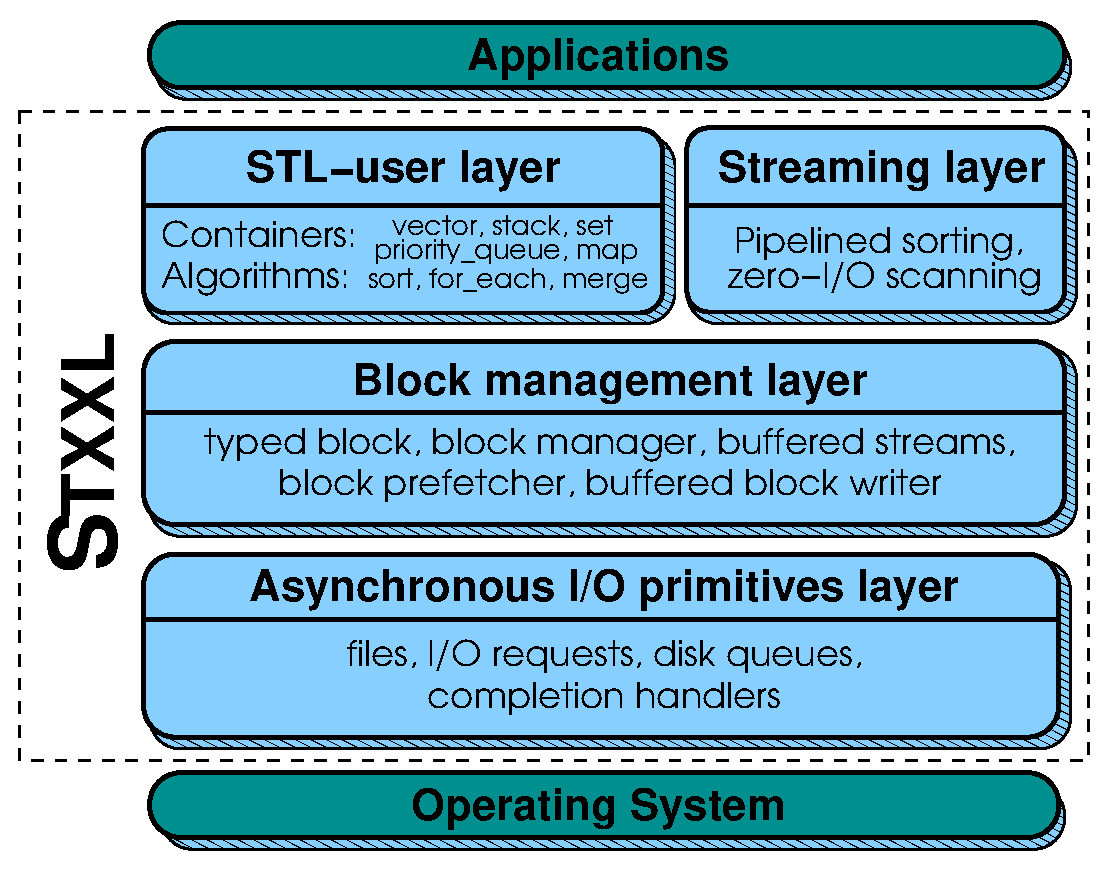
\includegraphics[width=8cm]{logo1}
\end{center}
\vspace*{-0.3cm}
\caption{\label{stxxlstructure}The \stxxl library structure}
\end{figure}

The middle layer, \emph{Block management layer} provides a programming
interface simulating the \emph{parallel} disk model. The layer provides
abstraction for a fundamental concept in the external memory algorithm
design -- block of elements. Block manager implements
block allocation/deallocation allowing several block-to-disk
assignment strategies: striping, randomized striping, randomized
cycling, etc. The block management layer provides implementation
of \emph{parallel} disk buffered writing and optimal prefetching
\cite{HutSanVit01b}, and block caching. The implementations are fully
asynchronous and designed to explicitly support overlapping of I/O
and computation. 

The top of \stxxl consists of two modules (see Fig.~\ref{stxxlstructure}). 
STL-user layer implements the functionality and interfaces of the STL
library. The layer provides external memory sorting, external memory
stack, external memory priority queue, etc. which have
(almost) the same interfaces (including syntax and semantics) as their
STL counterparts.

The \emph{Streaming layer} provides efficient support for external
memory algorithms with mostly \emph{sequential} I/O pattern, i.e.\ scan, sort,
merge, etc. A user algorithm, implemented using this module can save
many I/Os\footnote{The doubling algorithm for external memory suffix
array construction implemented with this module requires only $1/3$ of
I/Os which must be performed by an implementation that uses conventional
data structures and algorithms (from \stxxl STL-user layer, or LEDA-SM,
or TPIE).}. The win is due to an efficient interface, that couples the
input   
and the output of the algorithms-components (scans, sorts,
etc.). The 
output from an algorithm is directly fed into another algorithm as the
input, without the need to store it on the disk.


\chapter{STL-User Layer}
\stxxl library was designed to ease the access to external memory
algorithms and data structures for a programmer. We decided to
equip our implementations of \emph{out-of-memory} data structure and
algorithms with well known generic interfaces of \emph{internal memory}
data structures and algorithms from the Standard Template Library.
Currently we have implementation of the following data structures (in
STL terminology \emph{containers}):
\texttt{vector}, \texttt{stack}, \texttt{priority\_queue}. We
have implemented a \emph{parallel} disk sorter which have syntax of
STL \texttt{sort} \cite{DemSan03}. Our \texttt{ksort} is a specialized
implementation 
of \texttt{sort} which efficiently sorts elements with integer
keys\footnote{\texttt{ksort} is not STL compatible, it extends the
syntax of STL.}. \stxxl currently provides several implementations of
scanning algorithms (\texttt{generate}, \texttt{for\_each},
\texttt{find}) optimized for external memory. However, it is possible
(with some constant factor degradation in the performance) to apply
internal memory scanning algorithms from STL to \stxxl 
containers, since \stxxl containers have iterator based interface.

\stxxl has a restriction that the data types stored in the containers
can not have pointers or references to other elements of external memory
containers. The reason is that those pointers/references get
invalidated when the blocks containing the elements they point/refer to are
written on the disks.


\newcommand{\xvector}{\texttt{stxxl::vector}}

\section{Vector}
External memory vector (array)
\xvector\ is a data structure 
that supports random access to elements. The semantics of the basic
methods of \xvector\ is kept to compatible with STL
\texttt{std::vector}. Table~\ref{rtvector} shows the internal work and
the I/O worst case complexity of the \xvector.

\begin{table}
\begin{center}
\caption{Running times of the basic operations of \xvector}
\label{rtvector}
\begin{tabular}{|l|c|c|}
\hline
                    & int. work & I/O (worst case) \\
\hline\hline
random access       & $\Oh{1}$ & $\Oh{1}$\\
\hline
insertion at the end& $\Oh{1}$ & $\Oh{1}$\\
\hline
removal at the end  & $\Oh{1}$ & $\Oh{1}$ \\
\hline
\end{tabular}
\end{center}
\end{table}

\subsection{The Architecture of \xvector}
The \xvector\ is organized as a collection of blocks residing on the
external storage media (parallel disks). Access to the external blocks
is organized through the fully associative \emph{cache} which consist of some
fixed amount of in-memory pages\footnote{The page is a collection of
consecutive blocks. The number of blocks in the page is
constant.}. The schema of 
\xvector\ is depicted 
in the Fig.~\ref{xvectorschema}. When accessing an element the
implementation of \xvector\ access methods (\texttt{[$\cdot$]}~operator,
\texttt{push\_back}, etc.) first checks
whether the page to which the requested element belongs is in the
vector's cache. If it is the case the reference to the
element in the cache is returned. Otherwise the page is brought into the
cache\footnote{If the page of the element has not been touched so 
far, this step is skipped. To keep an eye on such situations there is a
special flag 
for each page.}. If there was no free space in the cache, then some
page is to be written out. Vector maintains a \emph{pager} object, that
tells which page to kick out. \stxxl provides LRU and random paging
strategies. The most efficient and default one is LRU. For each page
vector maintains the \emph{dirty} flag, which is set when
\emph{non-constant} reference to one of the page's elements was
returned. The dirty flag 
is cleared each time when the page is read into the cache. The purpose of the
flag is to track whether any element of the page is modified and
therefore the page needs to
be written to the disk(s) when it has to be evicted from the
cache. 

\begin{figure}[hb]
\begin{center}
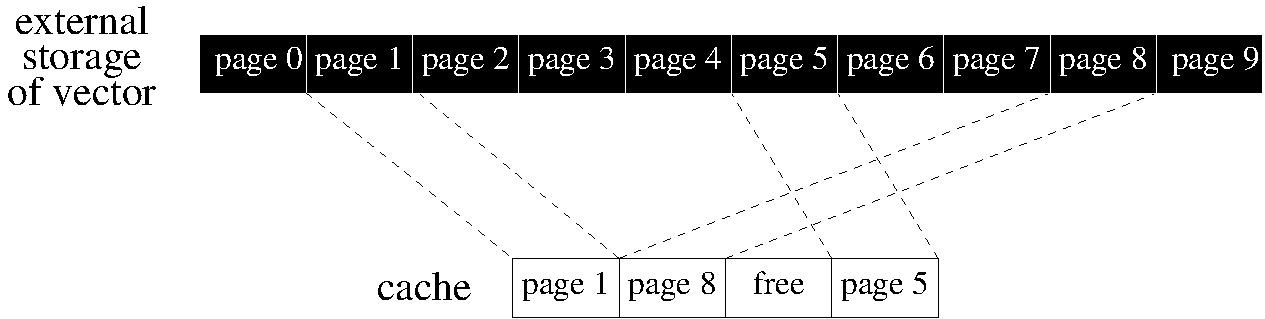
\includegraphics[width=11cm]{vector}
\end{center}
\vspace*{-0.3cm}
\caption{\label{xvectorschema} The schema of \xvector\ that consists
of ten external memory pages and has a cache with the capacity of four
pages. The 
first cache page is mapped to external page 1, the second page
is mapped to external page 8, and the fourth cache page is
mapped to page 5. The third page is not assigned to any external
memory page. }
\end{figure}

In the worst case scenario when vector elements are
read/written in the random order each access takes $2 \times
blocks\_per\_page$ I/Os. The factor \emph{two} shows up here because one has
to write the replaced from cache page and read the required
one). However the scanning of the array costs about $n/B$ I/Os using
constant vector iterators or const reference to the
vector\footnote{$n$ is the number of elements to read or write.}
(read-only 
access). Using non-const vector access methods leads to $2 \times n/B$
I/Os because every page becomes dirty when returning a non const
reference. 
If one needs only to sequentially write elements to the vector in
$n/B$ I/Os the 
currently fastest method is \texttt{stxxl::generate} (see section
\ref{stxxl::generate}). Sequential writing to an untouched before 
vector\footnote{For example writing in the vector that has been
created using 
\texttt{vector(size\_type n)} constructor.} or alone 
adding elements at the end of the vector\footnote{Using \texttt{void
push\_back(const T\&)} method.} leads also to $n/B$ I/Os.  

{\bf Example of use}
\begin{lstlisting}
stxxl::vector<int> V;
V.push_back(3);
assert(V.size() == 1 && V.capacity() >= 1 && V[0] == 3);
\end{lstlisting}

\newcommand{\xvectorg}{\texttt{stxxl::VECTOR\_GENERATOR}}

\subsection{\xvectorg}


Besides the type of the elements \xvector\ has many other template parameters
(block size, number of blocks per page, pager class, etc.). To make
the configuration of the vector type easier \stxxl
provides special type generator template meta programs for its
containers.  

The program
for \xvector\ is called \xvectorg.

{\bf Example of use}
\begin{lstlisting}
typedef stxxl::VECTOR_GENERATOR<int>::result vector_type;
vector_type V;
V.push_back(3);
assert(V.size() == 1 && V.capacity() >= 1 && V[0] == 3);
\end{lstlisting}

\begin{table}[h]
\begin{center}
\caption{Template parameters of \xvectorg\ from left to right.}
\label{vectorparam}
\begin{tabular}{|l|p{3.5cm}|c|c|}
\hline
parameter& description  & default value & recommended value \\
\hline\hline
Tp\_       & element type & & \\
\hline
PgSz\_     & number of blocks in a 
page
& 4 & $\geq D$\\
\hline
Pages\_    & number of pages in the cache & 8 & $\geq 2$ \\
\hline
BlkSize\_  & block size $B$ in bytes & $2\times 1024\times 1024$ & larger
is better\\
\hline
AllocStr\_ & parallel disk assignment strategy 
(Table~\ref{allocstr})
& RC & RC \\
\hline
Pager\_ & paging strategy 
(Table~\ref{pagingstr})
& lru & lru \\
\hline
\end{tabular}
\end{center}
\end{table}


%%\texttt{stxxl::VECTOR\_GENERATOR< Tp,\\ PgSz,\\ Pages,\\ BlkSize,\\
%%AllocStr,\\ Pager >} 

\begin{table}[h]
\begin{center}
\caption{Supported parallel disk assignment strategies.}
\label{allocstr}
\begin{tabular}{|l|c|}
\hline
strategy & identifier  \\
\hline\hline
striping & striping \\
\hline
simple randomized & SR\\
\hline
fully randomized & FR\\
\hline
randomized cycling & RC \\
\hline
\end{tabular}
\end{center}
\end{table}

\begin{table}[h]
\begin{center}
\caption{Supported paging strategies.}
\label{pagingstr}
\begin{tabular}{|l|c|}
\hline
strategy & identifier  \\
\hline\hline
random & random \\
\hline
least recently used & lru\\
\hline
\end{tabular}
\end{center}
\end{table}

Notes:
\begin{itemize}
\item All blocks of a page are read and written from/to
disks together. Therefore to increase the I/O bandwidth, it is
recommended to set the PgSz\_ parameter to multiple of $D$.
\end{itemize}

Since there are defaults for the last five
of the parameters, it is not necessary to specify them all.
{\bf Examples:}
\begin{itemize}
\item \texttt{VECTOR\_GENERATOR<double>::result} -- external vector of
{\bf double}'s with four blocks per page, the cache with eight pages, 2~MB
blocks, Random  Allocation and lru cache replacement strategy 
\item \texttt{VECTOR\_GENERATOR<double,8>::result} -- external vector
of {\bf double}'s , with {\bf eight} blocks per page, the cache with eight pages, 2~MB
blocks, Random  Allocation and lru cache replacement strategy 
\item \texttt{VECTOR\_GENERATOR<double,8,2,524288,SR>::result} --
external vector of {\bf double}'s, with {\bf eight} blocks per page, the cache
with {\bf two} pages, {\bf 512~KB} 
blocks, {\bf Simple Randomized} allocation and lru cache replacement strategy 
\end{itemize}

\subsection{Internal Memory Consumption of \xvector}
The cache of \xvector\ largely dominates in its internal memory
consumption. Other members consume very small fraction of \xvector s
memory even when the vector size is large. Therefore, the internal
memory consumption of \xvector\ can be estimated as
$BlkSize\_ \times Pages\_ \times PgSz\_$ bytes.



\subsection{Members of \xvector}
See Tables \ref{vectormembers1} and  \ref{vectormembers2}.

\begin{table}[h]
\begin{center}
\caption{Members of \xvector. Part 1.}
\label{vectormembers1}
\begin{tabular}{|p{6cm}|p{5cm}|}
\hline
member & description  \\
\hline\hline
\texttt{value\_type} &  The type of object, Tp\_, stored in the vector. \\
\hline
\texttt{pointer} & Pointer to Tp\_. \\
\hline
\texttt{reference} & Reference to Tp\_. \\
\hline
\texttt{const\_reference} & Const reference to Tp\_. \\
\hline
\texttt{size\_type} & An unsigned 64-bit\footnote{\texttt{off\_t}
type. It has the length 64 bits if \ldots} integral type. \\
\hline
\texttt{iterator} & Iterator used to iterate through a vector. See
notes a,b. \\
\hline
\texttt{const\_iterator} & Const iterator used to iterate through a
vector. See notes a,b. \\
\hline
\texttt{block\_type} & type of the block used in disk-memory 
transfers \\
\hline
\texttt{iterator begin()} & Returns an iterator pointing to the
beginning of the vector. See notes a,b. \\
\hline
\texttt{iterator end()} & Returns an iterator pointing to the end of
the vector. See notes a,b.\\
\hline
\texttt{const\_iterator begin() const} & Returns a const\_iterator
pointing to the beginning of the vector. See notes a,b.\\ 
\hline
\texttt{const\_iterator end() const} & Returns a const\_iterator
pointing to the end of the vector. See notes a,b. \\
\hline
\texttt{size\_type size() const} & Returns the size of the vector. \\
\hline
\texttt{size\_type capacity() const} & Number of elements for which
\emph{external} memory has been allocated. \texttt{capacity()} is always
greater than or equal to \texttt{size()}. \\
\hline
\texttt{bool empty() const} & true if the vector's size is 0.\\
\hline
\texttt{reference operator[](size\_type n)} & Returns (the reference to)
the n'th element. See note c.\\ 
\hline
\texttt{const\_reference operator[](size\_type n) const} & Returns
(the const reference to)
the n'th element. See note c.\\ 
\hline
\end{tabular}
\end{center}
\end{table}

\begin{table}[h]
\begin{center}
\caption{Members of \xvector. Part 2.}
\label{vectormembers2}
\begin{tabular}{|p{6cm}|p{5cm}|}
\hline
member & description  \\
\hline\hline
\texttt{vector()} & Creates an empty vector. \\
\hline
\texttt{vector(size\_type n)} & Creates a vector with n elements. \\
\hline
\texttt{vector(const vector\&)} & Not yet implemented \\
\hline
\texttt{\textasciitilde vector()} & The destructor. \\
\hline
\texttt{void reserve(size\_type n)} & If n is less than or equal to
\texttt{capacity()}, this call has no effect. Otherwise, it is a request for
allocation of additional \emph{external} memory. If the request is successful, then
\texttt{capacity()} is greater than or equal to n; otherwise,
\texttt{capacity()} is 
unchanged. In either case, \texttt{size()} is unchanged. \\
\hline
\texttt{reference front()} & Returns (the reference to) the first
element. See note c.\\
\hline
\texttt{const\_reference front() const} & Returns (the const reference to)
the first element. See note c.\\ 
\hline
\texttt{reference back()} & Returns (the reference to) the last
element. See note c.\\
\hline
\texttt{const\_reference back() const} & Returns (the const reference to)
the last element. See note c.\\ 
\hline
\texttt{void push\_back(const T\&)} & Inserts a new element at the
end. \\
\hline
\texttt{void pop\_back()} & Removes the last element. \\
\hline
\texttt{void clear()} & Erases all of the elements and deallocates all
external memory that vector occupied.\\
\hline
\texttt{void flush()} & Flushes the cache pages to the external
memory. \\
\hline
\texttt{vector (file * from)} & Create the vector from the
file. The construction causes no I/O.\\
\hline
\end{tabular}
\end{center}
\end{table}


Notes:
\begin{enumerate}
\item In opposite to STL, \xvector 's iterators do not get invalidated
when the vector is resized or reallocated.
\item Dereferencing a non-const iterator makes the page of the element
to which the iterator points to \emph{dirty}. This causes the page to
be written back to the disks(s) when the page is to be kicked off from
the cache (additional write I/Os). If you do not want this behavior,
use const iterators instead. Example:
\begin{lstlisting}
vector_type V;

// ... fill the vector here

vector_type::iterator iter = V.begin();

// ... advance the iterator
a = *iter; // causes write I/Os,
           // although *iter is not changed
vector_type::const_iterator citer = V.begin();
// ... advance the iterator
a = *citer; // read-only access, causes no write I/Os
*citer = b; // does not compile, citer is const

\end{lstlisting}
\item Non const \texttt{[$\cdot$]} operator makes the page of the
element \emph{dirty}. This causes the page to
be written back to the disks(s) when the page is to be kicked off from
the cache (additional write I/Os). If you do not want this behavior,
use const \texttt{[$\cdot$]} operator. For that you need to access the
vector via a const reference to it. Example:
\begin{lstlisting}
vector_type V;

// ... fill the vector here

a = V[index]; // causes write I/Os, 
              // although V[index] is not changed

const vector_type & CV = V; // const reference to V
a = CV[index]; // read-only access, can cause no write I/Os
CV[index] = b; // does not compile, CV is const
\end{lstlisting}
This issue also concerns \texttt{front()} and \texttt{back()} methods.
\end{enumerate}

\newcommand{\xstack}{\texttt{stxxl::stack}}

\section{Stacks}
\label{stacksection}
Stacks provide only restricted subset of
sequence operations: insertion, removal, and inspection of the element
at the top of the stack. Stacks are a "last in first out" (LIFO) data
structures: the element at the top of a stack is the one that was most
recently added. Stacks does not allow iteration through its
elements. 

The \emph{I/O efficient} stack is perhaps the simplest external memory
data structure. The basic variant of EM stack keeps the top $k$
elements in the main memory buffer, where $k \leq 2B$. If the buffers
get empty on a removal call, one block is brought from the disk to the
buffers. Therefore at least $B$ removals are required to make one I/O
reading a block. Insertions cause no I/Os until the internal buffers
get full. In this case to make space the first $B$ elements are
written to the disk. Thus a block write happens only after at least
$B$ insertions. If we choose the unit of disk
transfer to be a multiple of $DB$ (we denote it as a \emph{page}), set the
stack buffer size to $2D$ pages, and evenly assign the blocks of a
page to disks we obtain the running times shown in
Table~\ref{rtstack}. 

\begin{table}[h]
\begin{center}
\caption{Amortized running times of the basic operations of \xstack}
\label{rtstack}
\begin{tabular}{|l|c|c|}
\hline
                    & int. work & I/O (amortized)\\
\hline\hline
insertion at the end& $\Oh{1}$ & $\Oh{1/DB}$\\
\hline
removal at the end  & $\Oh{1}$ & $\Oh{1/DB}$ \\
\hline
\end{tabular}
\end{center}
\end{table}

\stxxl has several implementations of the external memory stack. Each 
implementation is specialized for a certain access pattern:
\begin{itemize}
\item The {\bf Normal } stack (\texttt{stxxl::normal\_stack}) is a general
purpose implementation which is the best if the access pattern
to the stack is an irregular mix of push'es and pop's, i.e.\ the stack
grows and shrinks without a certain rule.
\item The {\bf Grow-Shrink} stack is a stack that is optimized for an
access pattern where the insertions are (almost) not intermixed with
the removals, and/or vice versa, the removals are (almost) not
intermixed with the insertions. In other words the stack first grows
to its maximal size, then it shrinks, then it might again grow, then
shrink, and so forth, i.e.\ the pattern is
$(push^{i_j}pop^{r_j})^k$, where $k \in N$, $1\leq j\leq k$, and
$i_j$, $r_j$ are \emph{large}. 
\item The {\bf Grow-Shrink2} stack is a ``grow-shrink'' stack that
allows the use of common prefetch and write buffer pools. The pools
are shared between several ``grow-shrink'' stacks.
\item The {\bf Migrating} stack is a stack that migrates from
internal memory to external when its size exceeds a certain
threshold. 
% todo: describe the optimization in its section later
\end{itemize}

\newcommand{\xnormalstack}{\texttt{stxxl::normal\_stack}}
\subsection{\xnormalstack}
The \xnormalstack is a general purpose implementation of the external
memory stack. The stack has two pages, the size of the page in blocks
is a configuration constant and can be given as a template
parameter. The implementation of the methods follows the description
given in Section~\ref{stacksection}.

\subsection*{Internal Memory Consumption of \xnormalstack}
The cache of \xnormalstack\ largely dominates in its internal memory
consumption. Other members consume very small fraction of
\xnormalstack s 
memory even when the stack size is large. Therefore, the internal
memory consumption of \xnormalstack\ can be estimated as
$2 \times BlkSize\_ \times PgSz\_$ bytes, where $BlkSize\_$ is the
block size and $PgSz\_$ is the page size in blocks (see
Section~\ref{stackgensection}). 

\subsection*{Members of \xnormalstack}
See Table~\ref{normalstackmembers}.

\begin{table}[h]
\begin{center}
\caption{Members of \xnormalstack.}
\label{normalstackmembers}
\begin{tabular}{|p{6cm}|p{5cm}|}
\hline
member & description  \\
\hline\hline
\texttt{value\_type} &  The type of object, Tp\_, stored in the vector. \\
\hline
\texttt{size\_type} & An unsigned 64-bit\footnote{\texttt{off\_t}
type. It has the length 64 bits if \ldots} integral type. \\  
\hline
\texttt{block\_type} & type of the block used in disk-memory 
transfers \\
\hline
\texttt{bool empty() const} &  Returns true if the stack contains no
elements, and false  otherwise. \texttt{S.empty()} is equivalent to \texttt{S.size() ==
0}. \\ 
\hline
\texttt{size\_type size() const} & Returns the number of elements
contained in the stack. \\
\hline
\texttt{value\_type\& top()} & Returns a mutable reference to the
element at the top of the stack. Precondition: \texttt{empty()} is
false. \\ 
\hline
\texttt{const value\_type\& top() const} & Returns a const reference
to the element at the top of the stack. Precondition: \texttt{empty()} is
false.\\ 
\hline
\texttt{void push(const value\_type\& x)} & Inserts x at the top of
the stack. Postconditions: \texttt{size()} will be incremented by 1,
and \texttt{top()} will be equal to x. \\
\hline
\texttt{void pop()} & Removes the element at the top of the stack.
Precondition: \texttt{empty()} is false. Postcondition: size() will be
decremented by 1. \\ 
\hline
\texttt{normal\_stack()} & he default constructor. Creates an empty
stack.\\
\hline
\texttt{template <class stack\_type>
normal\_stack(const stack\_type \& stack\_)} & The copy
constructor. Accepts any \emph{stack concept} data type.\\ 
\hline
\texttt{\textasciitilde normal\_stack()} & The destructor.\\
\hline
\end{tabular}
\end{center}
\end{table}

The running times of the push/pop
stack operations are given in Table~\ref{rtstack}. Other operations
except copy construction perform constant internal work and no I/Os.

\newcommand{\xgsstack}{\texttt{stxxl::grow\_shrink\_stack}}
\subsection{\xgsstack}
The \xgsstack\ stack specialization is optimized for an
access pattern where the insertions are (almost) not intermixed with
the removals, and/or vice versa, the removals are (almost) not
intermixed with the insertions. In other words the stack first grows
to its maximal size, then it shrinks, then it might again grow, then
shrink, and so forth, i.e.\ the pattern is
$(push^{i_j}pop^{r_j})^k$, where $k \in N$, $1\leq j\leq k$, and
$i_j$, $r_j$ are \emph{large}. 
The implementation efficiently exploits the knowledge of the access
pattern that allows \emph{prefetching} the blocks beforehand while the stack
shrinks and \emph{buffered writing} while the stack grows. Therefore
the \emph{overlapping} of I/O and computation is possible.

\subsection*{Internal Memory Consumption of \xgsstack}
The cache of \xgsstack\ largely dominates in its internal memory
consumption. Other members consume very small fraction of
\xgsstack 's 
memory even when the stack size is large. Therefore, the internal
memory consumption of \xgsstack\ can be estimated as
$2 \times BlkSize\_ \times PgSz\_$ bytes, where $BlkSize\_$ is the
block size and $PgSz\_$ is the page size in blocks (see
Section~\ref{stackgensection}). 

\subsection*{Members of \xgsstack}
The \xgsstack has the same set of members as the \xnormalstack\  (see
Table~\ref{normalstackmembers}). The running times of \xgsstack\ are the
same as \xnormalstack\ except that when the stack switches from
growing to shrinking (or from shrinking to growing) $PgSz\_$ I/Os can
be spent additionally in the worst case.\footnote{This is for the single
disk setting, if the page is perfectly striped over parallel disk the
number of I/Os is $PgSz\_/D$.}

\newcommand{\xgsstacktwo}{\texttt{stxxl::grow\_shrink\_stack2}}
\subsection{\xgsstacktwo}
The \xgsstacktwo\ is optimized for the same kind of access pattern as
\xgsstack. The difference is that each instance of \xgsstack\ uses
an own internal buffer to overlap I/Os and computation, but
\xgsstacktwo\ is able to share the buffers from the pool used by
several stacks. 

% mention the documentation of prefetch\_pool and write\_pool.

\subsection*{Internal Memory Consumption of \xgsstacktwo}
Not counting the memory consumption of the shared blocks from the
pools, the stack alone consumes about $BlkSize\_$ bytes.\footnote{It has
the cache that consists of only a single block.}

\subsection*{Members of \xgsstacktwo}
The \xgsstacktwo\ has almost the same set of members as the
\xnormalstack\
(Table~\ref{normalstackmembers}), except that it does not have the
default constructor. The \xgsstacktwo\ requires
prefetch and write pool objects (see Sections
\ref{prefetchpoolsection} and \ref{writepoolsection} for the
documentation for the pool classes) to be specified in the creation
time. 
The new members are listed in Table~\ref{gsstacktwomembers}.

\begin{table}[h]
\begin{center}
\caption{New members of \xgsstacktwo.}
\label{gsstacktwomembers}
\begin{tabular}{|p{6cm}|p{5cm}|}
\hline
member & description  \\
\hline\hline
\texttt{grow\_shrink\_stack2 (prefetch\_pool< block\_type > \&
p\_pool\_, write\_pool< block\_type > \&w\_pool\_, unsigned
prefetch\_aggressiveness=0)} &  Constructs stack, that will use
\texttt{p\_pool\_} for prefetching and \texttt{w\_pool\_} for buffered
writing. \texttt{prefetch\_aggressiveness} parameter tells how many
blocks from the prefetch pool the stack is allowed to use.\\  
\hline
\texttt{void set\_prefetch\_aggr (unsigned new\_p)} & Sets level of
prefetch aggressiveness (number of blocks from the prefetch pool used
for prefetching). \\
\hline
\texttt{unsigned get\_prefetch\_aggr () const} & Returns the number of
blocks used for prefetching. \\
\hline
\end{tabular}
\end{center}
\end{table}


\newcommand{\xmstack}{\texttt{stxxl::migrating\_stack}}
\subsection{\xmstack}
The \xmstack\ is a stack that migrates from internal memory to
external when its size exceeds a certain threshold (template
parameter). The implementation
of internal and external memory stacks can be arbitrary and given as a
template parameters.


\subsection*{Internal Memory Consumption of \xmstack}
The \xmstack\ memory consumption depends on the memory consumption of
the stack implementations given as template parameters. The the
current state is internal (external), the \xmstack\ consumes almost
exactly the same space as internal (external) memory stack
implementation.\footnote{The \xmstack\ needs only few pointers to
maintain the switching from internal to external memory
implementations.}  

\subsection*{Members of \xmstack}
The \xmstack\ extends the member set of \xnormalstack\
(Table~\ref{normalstackmembers}). The new members are listed in
Table~\ref{migratingstackmembers}. 
\begin{table}[h]
\begin{center}
\caption{New members of \xmstack.}
\label{migratingstackmembers}
\begin{tabular}{|p{6cm}|p{5cm}|}
\hline
member & description  \\
\hline\hline
\texttt{bool    internal () const} & Returns true if the current
implementation is internal, otherwise false. \\ 
\hline
\texttt{bool    external () const} & Returns true if the current
implementation is external, otherwise false. \\
\hline
\end{tabular}
\end{center}
\end{table}

\newcommand{\xstackg}{\texttt{stxxl::STACK\_GENERATOR}}

\subsection{\xstackg}
\label{stackgensection}

To provide an easy way to choose and configure the \xstack\
implementations \stxxl offers a template meta program called
\xstackg. See Table~\ref{stackparam}.

{\bf Example:}
\begin{lstlisting}
typedef stxxl::STACK_GENERATOR<int>::result stack_type;

int main()
{
  stack_type S;
  S.push(8);
  S.push(7);
  S.push(4);
  assert(S.size() == 3);

  assert(S.top() == 4);
  S.pop();

  assert(S.top() == 7);
  S.pop();

  assert(S.top() == 8);
  S.pop();

  assert(S.empty());
}

\end{lstlisting}

\begin{table}[h]
\begin{center}
\caption{Template parameters of \xstackg\ from left to right.}
\label{stackparam}
\begin{tabular}{|l|p{4.5cm}|c|c|}
\hline
parameter& description  & default value & recommended value \\
\hline\hline
ValTp       & element type & & \\
\hline
Externality & tells whether the vector is internal, external, or
migrating (Table~\ref{externality}) & external & \\
\hline
Behavior & chooses \emph{external} implementation
(Table~\ref{behaviour})& normal & \\ 
\hline
BlocksPerPage & defines how many blocks has one page of internal cache
of an \emph{external} implementation & 4 &  $\geq D$ \\
\hline
BlkSz & external block size in bytes &  $2\times 1024\times 1024$ &
larger is better\\
\hline
IntStackTp & type of internal stack (used for the migrating stack) &  
\texttt{std::stack<ValTp>} &\\
\hline
MigrCritSize & threshold value for number of elements when
\texttt{migrating\_stack} migrates to the external memory & 
$2\times BlocksPerPage\times BlkSz$ & \\
\hline
AllocStr &  parallel disk assignment strategy 
(Table~\ref{allocstr}) & RC & RC \\
\hline
SzTp & size type & \texttt{off\_t} & \texttt{off\_t} \\
\hline
\end{tabular}
\end{center}
\end{table}


\begin{table}[h]
\begin{center}
\caption{The Externality parameter.}
\label{externality}
\begin{tabular}{|l|p{7cm}|}
\hline
identifier & comment \\
\hline\hline
internal & chooses IntStackTp implementation\\
\hline
external & external container, implementation is chosen according to
the Behavior parameter\\ 
\hline
migrating & migrates from internal implementation given by IntStackTp
parameter to external implementation given by Behavior parameter when
size exceeds MigrCritSize \\
\hline
\end{tabular}
\end{center}
\end{table}

\begin{table}[h]
\begin{center}
\caption{The Behavior parameter.}
\label{behaviour}
\begin{tabular}{|l|p{7cm}|}
\hline
identifier & comment \\
\hline\hline
normal & conservative version, implemented in \xnormalstack \\
\hline
grow\_shrink & chooses \xgsstack \\ 
\hline
grow\_shrink2 & chooses \xgsstacktwo \\
\hline
\end{tabular}
\end{center}
\end{table}


{\bf Example for \xgsstacktwo\ :}
\begin{lstlisting}

typedef STACK_GENERATOR<int,external,grow_shrink2>::result stack_type;
typedef stack_type::block_type block_type;

stxxl::prefetch_pool p_pool(10); // 10 read buffers
stxxl::write_pool w_pool(6);     // 6 write buffers
stack_type S(p_pool,w_pool,0);   // no read buffers used 

for(long long i=0;i < max_value;++i)
     S.push(i);
 
S.set_prefetch_aggressiveness(5); 
/* give a hint that we are going to
   shrink the stack from now on,
   always prefetch 5 buffers
   beforehand */

for(long long i=0; i< max_value;++i)
        S.pop();

S.set_prefetch_aggressiveness(0);
// stop prefetching 

\end{lstlisting}

\section{Priority Queue}
A priority queue is a data structure that provides a restricted subset of
container functionality: it provides insertion of elements, and
inspection and removal of the top element. It is guaranteed that the
top element is the largest element in the priority queue, where the
function object \texttt{Cmp\_} is used for comparisons.
Priority queue does not allow iteration through its elements. 

\newcommand{\xpqueue}{\texttt{stxxl::priority\_queue}}

\stxxl priority queue is an external memory implementation of
\cite{San00b}. The difference to the original design is that the
last merge groups keep their sorted sequences in the external memory.
The running times of \xpqueue\ data structure is given in
Table~\ref{rtpqueue}. The theoretic guarantees on I/O performance are
given only for a single disk setting, however the queue also performs
well in practice for multi-disk configuration.



\begin{table}[h]
\begin{center}
\caption{Amortized running times of the basic operations of \xpqueue{}
in terms of $I =$ the number of performed operations.}
\label{rtpqueue}
\begin{tabular}{|l|c|c|}
\hline
                    & int. work & I/O (amortized)\\
\hline\hline
insertion           & $\Oh{\log I}$ & $\Oh{1/B}$\\
\hline
deletion  & $\Oh{\log I}$ & $\Oh{1/B}$ \\
\hline
\end{tabular}
\end{center}
\end{table}

\subsection{Members of \xpqueue}
See Table~\ref{pqueuemembers}.

\begin{table}[h]
\begin{center}
\caption{Members of \xpqueue.}
\label{pqueuemembers}
\begin{tabular}{|p{6cm}|p{5cm}|}
\hline
member & description  \\
\hline\hline
\texttt{value\_type} &  The type of object, Tp\_, stored in the vector. \\
\hline
\texttt{size\_type} & An unsigned 64-bit\footnote{\texttt{off\_t}
type. It has the length 64 bits if \ldots} integral type. \\  
\hline
\texttt{block\_type} & type of the block used in disk-memory 
transfers \\
\hline
\texttt{priority\_queue( prefetch\_pool<block\_type>\& p\_pool\_, 
write\_pool<block\_type>\& w\_pool\_)} & Creates an empty priority
queue. Prefetch pool \texttt{p\_pool\_} and write pools
\texttt{w\_pool\_} will be used for overlapping of I/O and computation
during external memory merging (see Sections
\ref{prefetchpoolsection} and \ref{writepoolsection} for the
documentation for the pool classes).\\ 
\hline
\texttt{bool empty() const} & Returns true if the \texttt{priority\_queue}
contains no elements, and false  otherwise. \texttt{S.empty()} is
equivalent to \texttt{S.size() == 0}. \\ 
\hline
\texttt{size\_type size() const} & Returns the number of elements
contained in the \texttt{priority\_queue}. \\ 
\hline
\texttt{const value\_type\& top() const} & Returns a const reference to
the element at the top of the \texttt{priority\_queue}. The element at
the top 
is guaranteed to be the largest element in the priority queue, as
determined by the comparison function \texttt{Cmp\_}. That is, for
every 
other element x in the \texttt{priority\_queue}, \texttt{Cmp\_(Q.top(), x)} is
false. Precondition: \texttt{empty()} is false. \\
\hline
\texttt{void push(const value\_type\& x)}& Inserts x into the
\texttt{priority\_queue}. Postcondition: \texttt{size()} will be
incremented by 1.\\  
\hline
\texttt{void pop()} & Removes the element at the top of the
\texttt{priority\_queue}, that is, the largest element in the
\texttt{priority\_queue}. Precondition: \texttt{empty()} is
false. Postcondition: 
\texttt{size()} will be decremented by 1.  \\
\hline
\texttt{unsigned mem\_cons () const} & Returns number of bytes
consumed by the \texttt{priority\_queue} in the internal memory 
not including the pools.\\  
\hline
\texttt{\textasciitilde priority\_queue()} & The
destructor. Deallocates all occupied internal and external memory.\\
\hline
\end{tabular}
\end{center}
\end{table}


\newcommand{\xpqueueg}{\texttt{stxxl::PRIORITY\_QUEUE\_GENERATOR}}

\subsection{\xpqueueg}
Since the \xpqueue\ has many setup parameters (internal memory
buffer sizes, arity of mergers, number of internal and external memory
merger groups, etc.) which are difficult to guess, \stxxl\ provides a
helper meta template program 
that searches for the optimum settings for user demands. The program
is called \xpqueueg. The parameter of the program are given in
Table~\ref{pqueueparam}.

\begin{table}[h]
\begin{center}
\caption{Template parameters of \xpqueueg\ from left to right.}
\label{pqueueparam}
\begin{tabular}{|l|p{4.5cm}|c|c|}
\hline
parameter& description  & default value & recommended value \\
\hline\hline
Tp\_       & element type & & \\
\hline
Cmp\_ & the comparison type used to determine whether one element is
smaller than another element. See note a.& & \\ 
\hline
IntM\_ & upper limit for internal memory consumption in bytes & &
larges is better\\
\hline
MaxS\_ & upper limit for number of elements contained in the priority
queue (in units of 1024 items). See note b. & & \\ 
\hline
Tune\_ & a tuning parameter. See note c. & 6 &\\
\hline
\end{tabular}
\end{center}
\end{table}

Notes:
\begin{enumerate}
\item If \texttt{Cmp\_(x,y)} is true, then x is smaller than y. The element
returned by \texttt{Q.top()} is the largest element in the priority queue. That
is, it has the property that, for every other element x in the
priority queue, \texttt{Cmp\_(Q.top(), x)} is false. \texttt{Cmp\_}
must also provide 
\texttt{min\_value} method, that returns value of type \texttt{Tp\_}
that is smaller than 
any element of the queue x , i.e.\ \texttt{Cmp\_(Cmp\_.min\_value(),x))}
is always true. 

Example, a comparison object for priority queue where \texttt{top()}
returns the \emph{smallest} contained integer: 
\begin{lstlisting}
struct CmpIntGreater
{
  bool operator () (const int & a, const int & b)
  { return a<b; }
  int min_value() const  
  { return (std::numeric_limits<int>::max)(); }
};
\end{lstlisting}
Example, a comparison object for priority queue where \texttt{top()}
returns the \emph{largest} contained integer: 
\begin{lstlisting}
struct CmpIntLess: public std::less<int>
{
   int min_value() const  
   { return (std::numeric_limits<int>::min)(); }
};
\end{lstlisting}
Note that \texttt{Cmp\_} must define the Strict Weak Ordering.

\item Example: if you are sure that priority queue contains no more
than one million elements any time, then the right parameter for you is
$(1000000/1024)= 976$.

\item Try to play with the Tune\_ parameter if the your code does not
compile (larger than default value 6 might help). The reason that the
code does not 
compile is that no suitable 
internal parameters were found for given IntM\_ and MaxS\_. It might
also happen that given IntM\_ is too small for given MaxS\_, try larger
values.
 
\texttt{PRIORITY\_QUEUE\_GENERATOR} searches for 7 
configuration parameters of \xpqueue\ that both minimize
internal memory consumption of the priority queue to match IntM\_ and
maximize the performance of priority queue operations. Actual memory
consumption might be slightly larger (use
\texttt{stxxl::priority\_queue::mem\_cons()}
method to track it), since the search assumes rather optimistic
schedule of push'es and pop'es for the estimation of the maximum
memory consumption. To keep actual memory requirements low, increase
the value of MaxS\_ parameter. 
\item 
For the functioning, a priority queue object requires two pools of blocks
(See the constructor of \texttt{priority\_queue} ). To construct
\stxxl block pools 
you need the block type that is used by priority queue. Block's size
and hence it's type is generated by the 
\texttt{PRIORITY\_QUEUE\_GENERATOR} in compile type from IntM\_, MaxS\_
and \texttt{sizeof(Tp\_)} and it can not be given directly by the user
as a template parameter. The block type can be accessed as\\
\texttt{PRIORITY\_QUEUE\_GENERATOR<parameters>::result::block\_type}. 

\end{enumerate}

{\bf Example:}
\begin{lstlisting}
struct Cmp
{
  bool operator () (const int & a, 
                    const int & b) const 
  { return a>b; }
  int min_value() const  
  { return (std::numeric_limits<int>::max)(); }
};

typedef stxxl::PRIORITY_QUEUE_GENERATOR<int,
                                        Cmp,
/* use 64 MB on main memory */          64*1024*1024,
/* 1 billion items at most  */          1024*1024
                                        >::result pq_type;
typedef pq_type::block_type block_type;


int main() {
  // use 10 block read and write pools 
  // for enable overlapping of I/O and
  // computation
  stxxl::prefetch_pool<block_type> p_pool(10);
  stxxl::write_pool<block_type>    w_pool(10);

  pq_type Q(p_pool,w_pool);
  Q.push(1);
  Q.push(4);
  Q.push(2);
  Q.push(8);
  Q.push(5);
  Q.push(7);
  
  assert(Q.size() == 6);

  assert(Q.top() == 8);
  Q.pop();

  assert(Q.top() == 7);
  Q.pop();

  assert(Q.top() == 5);
  Q.pop();

  assert(Q.top() == 4);
  Q.pop();

  assert(Q.top() == 2);
  Q.pop();

  assert(Q.top() == 1);
  Q.pop();

  assert(Q.empty());
}


\end{lstlisting}

\subsection{Internal Memory Consumption of \xpqueue}
Internal memory consumption of \xpqueue\ is bounded by the IntM\_
parameter in most situations.

\newcommand{\xsort}{{\texttt{stxxl::sort}}}
\newcommand{\xksort}{{\texttt{stxxl::ksort}}}
\newcommand{\stdsort}{{\texttt{std::sort}}}



\section{\stxxl Algorithms}
Iterators of \xvector\ are STL
compatible. \texttt{stxxl::vector::iterator} is a model of Random
Access Iterator concept from STL. Therefore it is possible to use the
\xvector\ iterator ranges with STL algorithms. However such use is not
I/O efficient if an algorithm accesses the sequence in a random order.
For such kind of algorithms \stxxl provides I/O efficient
implementations described in this chapter
(Sections~\ref{sortsection}--\ref{ksortsection}). 
If an algorithm does only a scan (or a constant number of scans) of
a sequence (or sequences) the implementation that calls STL algorithm
is nevertheless I/O efficient. However one can save constant factors
in I/O volume 
and internal work if the the access pattern is known (read-only or
write-only scan for example). This knowledge is used in \stxxl
specialized implementations of STL algorithms
(Section~\ref{otheralgs}).

\subsection*{Example: STL Algorithms Running on \stxxl containers}
\begin{lstlisting}
typedef stxxl::VECTOR_GENERATOR<int>::result vector_type;

// Replace every number in an array with its negative.
const int N = 1000000000;
vector_type A(N);
std::iota(A.begin(), A.end(), 1);
std::transform(A, A+N, A, negate<double>());

// Calculate the sum of two vectors, 
// storing the result in a third vector.

const int N = 1000000000;
vector_type V1(N);
vector_type V2(N);
vector_type V3(N);

std::iota(V1.begin(), V1.end(), 1);
std::fill(V2.begin(), V2.end(), 75);

assert(V2.size() >= V1.size() && 
       V3.size() >= V1.size());
std::transform(V1.begin(), 
               V1.end(), 
               V2.begin(), 
               V3.begin(),
               plus<int>());
\end{lstlisting}

\section{Sorting}
\label{sortsection}
\xsort\ is an external memory equivalent to STL \stdsort.
The design and implementation of the algorithm is described in detail
in \cite{DemSan03}. 

\subsection*{Prototype}

\begin{lstlisting}
template < typename ExtIterator_, 
           typename StrictWeakOrdering_ 
         >
void sort ( ExtIterator_        first,
            ExtIterator_        last,
            StrictWeakOrdering_ cmp,
            unsigned            M
          )
\end{lstlisting}

\subsection*{Description}

\xsort\ sorts the elements in [first, last) into ascending order,
meaning 
that if \texttt{i} and \texttt{j} are any two valid iterators in
[first, last) such that 
\texttt{i} precedes \texttt{j}, then \texttt{*j} is not less than
\texttt{*i}. Note: as \stdsort, 
\xsort\ is not guaranteed to be stable. That is, suppose that
\texttt{*i} and \texttt{*j} are 
equivalent: neither one is less than the other. It is not guaranteed
that the relative order of these two elements will be preserved by
\xsort. 

The order is defined by the \texttt{cmp} parameter. The sorter's
internal memory consumption is bounded by \texttt{M} bytes.

\subsection*{Requirements on Types}

\begin{itemize}
\item \texttt{ExtIterator\_} is a model of External Random Access
Iterator\footnote{In \stxxl currently only \xvector\ provides
iterators that are models of External Random Access Iterator.}. 
\item \texttt{ExtIterator\_} is mutable.
\item \texttt{StrictWeakOrdering\_} is a model of Strict Weak Ordering
and must provide min and max values for the elements in the input:
 \begin{itemize}
 \item \texttt{max\_value} method that returns an object that is
   \emph{strictly greater} than all other objects of user type according
    to the given ordering. 
 \item \texttt{min\_value} method that returns an object that
    is \emph{strictly less} than all other objects of user type according
    to the given ordering.
 \end{itemize}
 {\bf Example:} 
  a comparison object for ordering integer elements in the ascending
  order
\begin{lstlisting}
struct CmpIntLess: public std::less<int>
{
   static int min_value() const  
   { return (std::numeric_limits<int>::min)(); }
   static int max_value() const  
   { return (std::numeric_limits<int>::max)(); }
};
 \end{lstlisting}
 {\bf Example:} 
  a comparison object for ordering integer elements in the descending
  order
\begin{lstlisting}
struct CmpIntGreater: public std::greater<int>
{
   int min_value() const  
   { return (std::numeric_limits<int>::max)(); }
   int max_value() const  
   { return (std::numeric_limits<int>::min)(); }
};
 \end{lstlisting}


 Note, that according to the \xsort\ requirements \texttt{min\_value}
and \texttt{max\_value} {\bf can not} be present in the input
sequence.
\item \texttt{ExtIterator\_}'s value type is convertible to
\texttt{StrictWeakOrdering\_}'s argument type.

\end{itemize}

\subsection*{Preconditions}
\label{sortpreconditions}
[first, last) is a valid range.

\subsection*{Complexity}
\label{sortcomplexity}
\begin{itemize}
\item Internal work: $\Oh{N \log N}$, where \\$N = (last -
first)\cdot$~\texttt{sizeof(ExtIterator\_::value\_type)}.
\item I/O complexity: $(2N/DB)(1 + \lceil {\log}_{M/B}(2N/M) \rceil)$ I/Os
\end{itemize}

\xsort\ chooses the block size (parameter $B$) equal to the block size
of the container, the last and first iterators pointing to
(e.g.\ \xvector's block size).

The second term in the I/O complexity accounts for the merge phases of
the external memory sorting algorithm \cite{DemSan03}. Avoiding
multiple merge phases  
speeds up the sorting. In practice one should choose the block size
$B$ of the container to be 
sorted such that there is only one merge phase needed: $\lceil
{\log}_{M/B}(2N/M) \rceil) = 1$. This is 
possible for $M > DB$ and $N < M^2/2DB$. But still this restriction
gives a freedom to choose a variety of blocks sizes. The study
\cite{DemSan03} has shown that optimal $B$ for sorting lies in the
range $[M^2/(4N),3M^2/(8N)]$. With such choice of the parameters the
\xsort\ always performs $4N/DB$ I/Os.

\subsection*{Internal Memory Consumption}
\label{sortimem}
The \xsort\ consumes slightly more than \emph{M} bytes of internal
memory. 

\subsection*{External Memory Consumption}
\label{sortemem}
The \xsort\ is not in-place. It requires about $N$ bytes of external
memory to store the sorted runs during the sorting process
\cite{DemSan03}. After the sorting this memory is freed.

\subsection*{Example}
\begin{lstlisting}
struct MyCmp: public std::less<int> // ascending
{                                   // order
   static int min_value() const  
   { return (std::numeric_limits<int>::min)(); }
   static int max_value() const  
   { return (std::numeric_limits<int>::max)(); }
};
typedef stxxl::VECTOR_GENERATOR<int>::result vec_type;

vec_type V;
// ... fill here the vector with some values

/*
   Sort in ascending order
   use 512 MB of main memory
*/
stxxl::sort(V.begin(),V.end(),MyCmp(),512*1024*1024);
// sorted
\end{lstlisting}

\section{Sorted Order Checking}
\stxxl gives an ability to automatically check the order in the output
of \stxxl \footnote{This checker checks the \xsort, \xksort\
(Section~\ref{ksortsection}), and 
the pipelined sorter from Section~\ref{pipesorting}.}
sorters and intermediate results of sorting (the order and a meta
information in the sorted runs). The check is switched on if the
source codes and the library are compiled with the option
\texttt{-DSTXXL\_CHECK\_ORDER\_IN\_SORTS} and the option
\texttt{-DNDEBUG} is not used. For details see the
\texttt{compiler.make} file in the \stxxl tar ball. Note, that the
checking routines require more internal work as well as additional $N/DB$
I/Os to read the sorted runs. Therefore for the final non-debug
version of a user application on should switch this option off.

%%%%%%%%%%%%%%%%%%%%%%%%%%%%%%%%%%%%%%%%%%%%%%%%%%%%%%%%%%%%%%%%%%%%%

\section{Sorting Using Integer Keys}
\label{ksortsection}
\xksort\ is a specialization of external memory sorting optimized for
records having integer keys.

\subsection*{Prototype}
\begin{lstlisting}
template < typename ExtIterator_>
void ksort ( ExtIterator_ first,
             ExtIterator_ last,
             unsigned     M
           )

template < typename ExtIterator_, typename KeyExtractor_>
void ksort ( ExtIterator_  first,
             ExtIterator_  last,
             KeyExtractor_ keyobj,
             unsigned      M
           )  
\end{lstlisting}

\subsection*{Description}
\xksort\ sorts the elements in [first, last) into ascending order,
meaning 
that if \texttt{i} and \texttt{j} are any two valid iterators in
[first, last) such that 
\texttt{i} precedes \texttt{j}, then \texttt{*j} is not less than
\texttt{*i}. Note: as \stdsort and \xsort, 
\xksort\ is not guaranteed to be stable. That is, suppose that
\texttt{*i} and \texttt{*j} are 
equivalent: neither one is less than the other. It is not guaranteed
that the relative order of these two elements will be preserved by
\xksort. 

The two versions of \xksort\ differ in how they define whether one
element is less than another. The first version assumes that 
the elements have \texttt{key()} member function that returns an
integral key (32 or 64 bit), as well as the minimum and the maximum
element values. The second version compares objects extracting the
keys using \texttt{keyobj} object, that is in turn provides min and
max element values.

The sorter's internal memory consumption is bounded by \texttt{M}
bytes. 

\subsection*{Requirements on Types}

\begin{itemize}
\item \texttt{ExtIterator\_} is a model of External Random Access
Iterator\footnote{In \stxxl currently only \xvector\ provides
iterators that are models of External Random Access Iterator.}. 
\item \texttt{ExtIterator\_} is mutable.
\item \texttt{KeyExtractor\_} must implement \texttt{operator ()} that
extracts the key of an element and provide min and max values for the
elements in the input: 
 \begin{itemize}
 \item \texttt{key\_type} typedef for the type of the keys.
 \item \texttt{max\_value} method that returns an object that is
   \emph{strictly greater} than all other keys of the elements in the
   input.  
 \item \texttt{min\_value} method that returns an object that
    is \emph{strictly less} than all other keys of the elements in the
    input.
 \end{itemize}
 {\bf Example:} 
  a key extractor object for ordering elements having 64 bit integer keys:
\begin{lstlisting}
struct MyType
{
   typedef unsigned long long key_type;
   key_type _key;
   char _data[32];
   MyType() {}
   MyType(key_type __key):_key(__key) {}
};
struct GetKey
{
   typedef MyType::key_type key_type;
   key_type operator() (const MyType & obj)
   { return obj._key; }
   MyType min_value() const 
   { return MyType(
        (std::numeric_limits<key_type>::min)()); }
   MyType max_value() const 
   { return MyType(
        (std::numeric_limits<key_type>::max)()); }
};
 \end{lstlisting}

 Note, that according to the \xsort\ requirements \texttt{min\_value}
and \texttt{max\_value} {\bf can not} be present in the input
sequence.
\item \texttt{ExtIterator\_}'s value type is convertible to
\texttt{KeyExtractor\_}'s argument type.

\item  \texttt{ExtIterator\_}'s value type has a typedef
\texttt{key\_type}. 

\item For the first version of \xksort\ \texttt{ExtIterator\_}'s value
type  must have the \texttt{key()} function that returns the key value
of the element, and the \texttt{min\_value()} and \texttt{max\_value()}
member functions that return minimum and maximum element values
respectively. Example:
\begin{lstlisting}
struct MyType
{
   typedef unsigned long long key_type;
   key_type _key;
   char _data[32];
   MyType() {}
   MyType(key_type __key):_key(__key) {}
   key_type key() { return _key; }
   MyType min_value() const 
   { return MyType(
        (std::numeric_limits<key_type>::min)()); }
   MyType max_value() const 
   { return MyType(
        (std::numeric_limits<key_type>::max)()); }
};
\end{lstlisting}

\end{itemize}

\subsection*{Preconditions}
The same as for \xsort\ (section~\ref{sortpreconditions}).

\subsection*{Complexity}
The same as for \xsort\ (Section~\ref{sortcomplexity}).

\subsection*{Internal Memory Consumption}
The same as for \xsort\ (Section~\ref{sortimem})

\subsection*{External Memory Consumption}
The same as for \xsort\ (Section~\ref{sortemem}).

\subsection*{Example}
\begin{lstlisting}
struct MyType
{
   typedef unsigned long long key_type;
   key_type _key;
   char _data[32];
   MyType() {}
   MyType(key_type __key):_key(__key) {}
   key_type key() { return obj._key; }
   static MyType min_value() const 
   { return MyType(
        (std::numeric_limits<key_type>::min)()); }
   static MyType max_value() const 
   { return MyType(
        (std::numeric_limits<key_type>::max)()); }
};

typedef stxxl::VECTOR_GENERATOR<MyType>::result vec_type;

vec_type V;
// ... fill here the vector with some values

/*
   Sort in ascending order
   use 512 MB of main memory
*/
stxxl::ksort(V.begin(),V.end(),512*1024*1024);
// sorted
\end{lstlisting}


%%%%%%%%%%%%%%%%%%%%%%%%%%%%%%%%%%%%%%%%%%%%%%%%%%%%%%%%%%%%%%%%%%%%
%%%%%%%%%%%%%%%%%%%%%%%%%%%%%%%%%%%%%%%%%%%%%%%%%%%%%%%%%%%%%%%%%%%%

\section{Other \stxxl Algorithms}
\label{otheralgs}

\stxxl offers several specializations of STL algorithms for \xvector\ 
iterators. The algorithms while accessing the elements bypass the
vector's cache and access the vector's blocks directly. Another
improvement is that algorithms from this chapter are able to overlap
I/O and computation. With standard STL algorithms the overlapping is
not possible. 
This measures save constant factors both in I/O volume and internal
work. 
%%%%%%%%%%%%%%%%%%%%%%%%%%%%%%%%%%%%%%%%%%%%%%%%%%%%%%%%%%%%%%%%%%%%5
\subsection{\texttt{stxxl::generate}}
\label{stxxl::generate}
The semantics of the algorithm is equivalent to the STL
\texttt{std::generate}. 

\subsection*{Prototype}
\begin{lstlisting}
template<typename ExtIterator, typename Generator>
void generate ( ExtIterator first,
                ExtIterator last,
                Generator gen,
                int nbuffers
              ) 
\end{lstlisting}
\subsection*{Description}
Generate assigns the result of invoking \texttt{gen}, a function
object that 
takes no arguments, to each element in the range [first, last). To
overlap I/O and computation \texttt{nbuffers} are used (a value at
least $D$ is recommended). The size of
the buffers is derived from the container that is pointed by the
iterators. 
\subsection*{Requirements on types}
\begin{itemize}
\item \texttt{ExtIterator} is a model of External Random Access
Iterator.
\item \texttt{ExtIterator} is mutable.
\item \texttt{Generator} is a model of STL Generator.
\item \texttt{Generator}'s result type is convertible to
\texttt{ExtIterator}'s 
value type.
\end{itemize}
\subsection*{Preconditions}
[first, last) is a valid range.
\subsection*{Complexity}
\begin{itemize}
\item Internal work is linear.
\item External work: close to $N/DB$ I/Os (write-only).
\end{itemize}

\subsection*{Example}
\begin{lstlisting}
// Fill a vector with random numbers, using the 
// standard C library function rand.
typedef stxxl::VECTOR_GENERATOR<int>::result vector_type;
vector_type V(some_size);
// use 20 buffer blocks
stxxl::generate(V.begin(), V.end(), rand, 20);
\end{lstlisting}
%%%%%%%%%%%%%%%%%%%%%%%%%%%%%%%%%%%%%%%%%%%%%%%%%%%%%%%%%%%%%%%%%%%%%%5
\newcommand{\xforeach}{{\texttt{stxxl::for\_each}}}
\subsection{\xforeach}
The semantics of the algorithm is equivalent to the STL
\texttt{std::for\_each}. 

\subsection*{Prototype}
\begin{lstlisting}
template<typename ExtIterator, typename UnaryFunction>
UnaryFunction for_each ( ExtIterator   first,
                         ExtIterator   last,
                         UnaryFunction f,
                         int nbuffers
                       )        
\end{lstlisting}
\subsection*{Description}
\xforeach\ applies the function object \texttt{f} to each element in the range
[first, last); \texttt{f}'s return value, if any, is
ignored. Applications are 
performed in forward order, i.e.\ from first to last. \xforeach\ returns
the function object after it has been applied to each element. 
 To
overlap I/O and computation \texttt{nbuffers} are used (a value at
least $D$ is recommended). The size of
the buffers is derived from the container that is pointed by the
iterators. 
\subsection*{Requirements on types}
\begin{itemize}
\item \texttt{ExtIterator} is a model of External Random Access
Iterator.
\item \texttt{UnaryFunction} is a model of STL Unary Function.
\item \texttt{UnaryFunction} does not apply any non-constant
operations through its argument.
\item \texttt{ExtIterator}'s value type is convertible to
\texttt{UnaryFunction}'s argument type.
\end{itemize}
\subsection*{Preconditions}
[first, last) is a valid range.
\subsection*{Complexity}
\begin{itemize}
\item Internal work is linear.
\item External work: close to $N/DB$ I/Os (read-only).
\end{itemize}
\subsection*{Example}
\begin{lstlisting}
template<class T> struct print : 
     public unary_function<T, void>
{
  print(ostream& out) : os(out), count(0) {}
  void operator() (T x) { os << x << ' '; ++count; }
  ostream& os;
  int count;
};
typedef stxxl::VECTOR_GENERATOR<int>::result vector_type;
int main()
{
  vector_type A(N);
  // fill A with some values
  // ...  

  print<int> P = stxxl::for_each(A.begin(), A.end(), 
                          print<int>(cout));
  cout << endl << P.count << " objects printed." << endl;
}
\end{lstlisting}
%%%%%%%%%%%%%%%%%%%%%%%%%%%%%%%%%%%%%%%%%%%%%%%%%%%%%%%%%%%%%%%%%%%%%%

\newcommand{\xforeachm}{{\texttt{stxxl::for\_each\_m}}}
\subsection{\xforeachm}
\xforeachm\ is a \emph{mutating} version of \xforeach, i.e.\ 
the restriction that Unary Function f can not apply any non-constant
operations through its argument does not exist.

\subsection*{Prototype}
\begin{lstlisting}
template<typename ExtIterator, typename UnaryFunction>
UnaryFunction for_each ( ExtIterator   first,
                         ExtIterator   last,
                         UnaryFunction f,
                         int nbuffers
                       )        
\end{lstlisting}
\subsection*{Description}
\xforeach\ applies the function object \texttt{f} to each element in the range
[first, last); \texttt{f}'s return value, if any, is
ignored. Applications are 
performed in forward order, i.e.\ from first to last. \xforeach\ returns
the function object after it has been applied to each element. 
 To
overlap I/O and computation \texttt{nbuffers} are used (a value at
least $2D$ is recommended). The size of
the buffers is derived from the container that is pointed by the
iterators. 
\subsection*{Requirements on types}
\begin{itemize}
\item \texttt{ExtIterator} is a model of External Random Access
Iterator.
\item \texttt{UnaryFunction} is a model of STL Unary Function.
\item \texttt{ExtIterator}'s value type is convertible to
\texttt{UnaryFunction}'s argument type.
\end{itemize}
\subsection*{Preconditions}
[first, last) is a valid range.
\subsection*{Complexity}
\begin{itemize}
\item Internal work is linear.
\item External work: close to $2N/DB$ I/Os (read and write).
\end{itemize}

\subsection*{Example}
\begin{lstlisting}
struct AddX
{
  int x;
  AddX(int x_): x(x_) {}
  void operator() (int & val)
  { val += x; }
};

typedef stxxl::VECTOR_GENERATOR<int>::result vector_type;
int main()
{
  vector_type A(N);
  // fill A with some values
  // ...  

  // Add 5 to each value in the vector
  stxxl::for_each(A.begin(), A.end(), AddX(5));
}
\end{lstlisting}
%%%%%%%%%%%%%%%%%%%%%%%%%%%%%%%%%%%%%%%%%%%%%%%%%%%%%%%%%%%%%%%%%5
\subsection{\texttt{stxxl::find}}
\label{stxxl::find}
The semantics of the algorithm is equivalent to the STL
\texttt{std::find}.

\subsection*{Prototype}
\begin{lstlisting}
template< typename ExtIterator, 
          typename EqualityComparable>
ExtIterator find ( ExtIterator                first,
                   ExtIterator                last,
                   const EqualityComparable & value,
                   int                        nbuffers
                 )  
\end{lstlisting}
\subsection*{Description}
Returns the first iterator \texttt{i} in the range [first, last) such
that \texttt{*i == value}. Returns last if no such iterator exists.  
To
overlap I/O and computation \texttt{nbuffers} are used (a value at
least $D$ is recommended). The size of
the buffers is derived from the container that is pointed by the
iterators. 

\subsection*{Requirements on types}
\begin{enumerate}
\item \texttt{EqualityComparable} is a model of STL EqualityComparable
concept.
\item \texttt{ExtIterator} is a model of External Random Access
Iterator. 
\item Equality is defined between objects  of type
\texttt{EqualityComparable} and objects of \texttt{ExtIterator}'s
value type.
\end{enumerate}
\subsection*{Preconditions}
[first, last) is a valid range.
\subsection*{Complexity}
\begin{itemize}
\item Internal work is linear.
\item External work: close to $N/DB$ I/Os (read-only).
\end{itemize}
\subsection*{Example}
\begin{lstlisting}
typedef stxxl::VECTOR_GENERATOR<int>::result vector_type;

vector_type V;
// fill the vector


// find 7 in V
vector_type::iterator result = find(V.begin(), V.end(), 7);
if(result != V.end())
 std::cout << ``Found at position ''<< 
      (result - V.begin()) << std::endl;
else
 std::cout << ``Not found'' << std::endl;
\end{lstlisting}
%%%%%%%%%%%%%%%%%%%%%%%%%%%%%%%%%%%%%%%%%%%%%%%%%%%%%%%%%%%%%%%%%%%
%%%%%%%%%%%%%%%%%%%%%%%%%%%%%%%%%%%%%%%%%%%%%%%%%%%%%%%%%%%%%%%%%%%

\chapter{Pipelined/Stream Interfaces}


%data flow graph, file, sorting, streaming nodes\\
%compare with TPIE AMI\_scan


\section{Preliminaries}
\section{Node Interface}
\section{Scheduling}
\section{File Nodes -- {\tt streamify} and {\tt materialize}}
\section{Streaming Nodes}
\section{Sorting Nodes}
\label{pipesorting}
\subsection{Runs Creator -- {\tt stxxl::stream::runs\_creator}}
\subsection{Specializations of {\tt stxxl::stream::runs\_creator}}
\subsection{Runs Merger --  {\tt stxxl::stream::runs\_merger}}
\subsection{A Combination: {\tt stxxl::stream::sort}}

\section{A Pipelined Version of the Billing Application}

\begin{lstlisting}

\end{lstlisting}

\chapter{Internals}
\section{Block Management Layer}

\subsection{\texttt{stxxl::prefetch\_pool}}
\label{prefetchpoolsection}
\subsection{\texttt{stxxl::write\_pool}}
\label{writepoolsection}

\section{I/O Primitives Layer}
\section{Utilities}


\chapter{Miscellaneous}
\section{\stxxl Compile Flags}

\bibliographystyle{plain} \bibliography{tutorial}

\end{document}
